\chapter{Measurement of Neutral Current Quasielastic
Interactions with Super-Kamiokande Gadolinium Upgrade}
\label{chp:ncqegd}

This chapter is dedicated to the main analysis of this thesis, the motivation for which is to constrain the SRN background by looking at the atmospheric neutral current quasi-elastic (NCQE) interactions of atmospheric neutrinos. The prompt and delayed signal of the NCQE interaction mimics that of the SRN, due to the positron providing the Cherenkov light of the prompt signal for SRN, while the prompt signal for NCQE is yielded by a gamma ray. The delayed capture process is the same for NCQE and SRN for captures on hydrogen, and prior to the Gd-loading, the NCQE neutron tag has searched for the 2.2 MeV photon from neutron capture on hydrogen. With the recent addition of 0.026\% $\mathrm{Gd}_{2}\left(\mathrm{SO}_{4}\right)_{3} \cdot 8 \mathrm{H}_{2} \mathrm{O}$ to Super-Kamiokande, neutron detection has improved due to the higher energy gamma cascade signal of neutron capture on gadolinium of 8 MeV. This At energies close to the atmospheric peak, the NCQE interaction cross sections can be evaluated using T2K beam neutrinos. This chapter will present the status of the improved neutron tag from SK-Gd, its impact on the measurement of NCQE in T2K and the improvements to the SRN background measurement.

There are many stages to this analysis, shown in Figure \ref{fig:analysis_flowchart}, where the ``neutron tagging'' stage occurs via two methods. Previously the NCQE neutron-tagging analyses used a method for neutron tagging which will be referred to as ``legacy NTag code'', but in 2020 the Super-K collaboration decided to proceed to use a new, more compact and streamlined version, which combines most of these stages into one piece of software. This will be referred to as``current NTag code'', and this is shown in Figure \ref{fig:analysis_flowchart} as well. The red arrows in Figure \ref{fig:analysis_flowchart} show the steps in the analysis prcoedure using the legacy NTag code which have been assimilated into the new NTag code.

\begin{figure}
    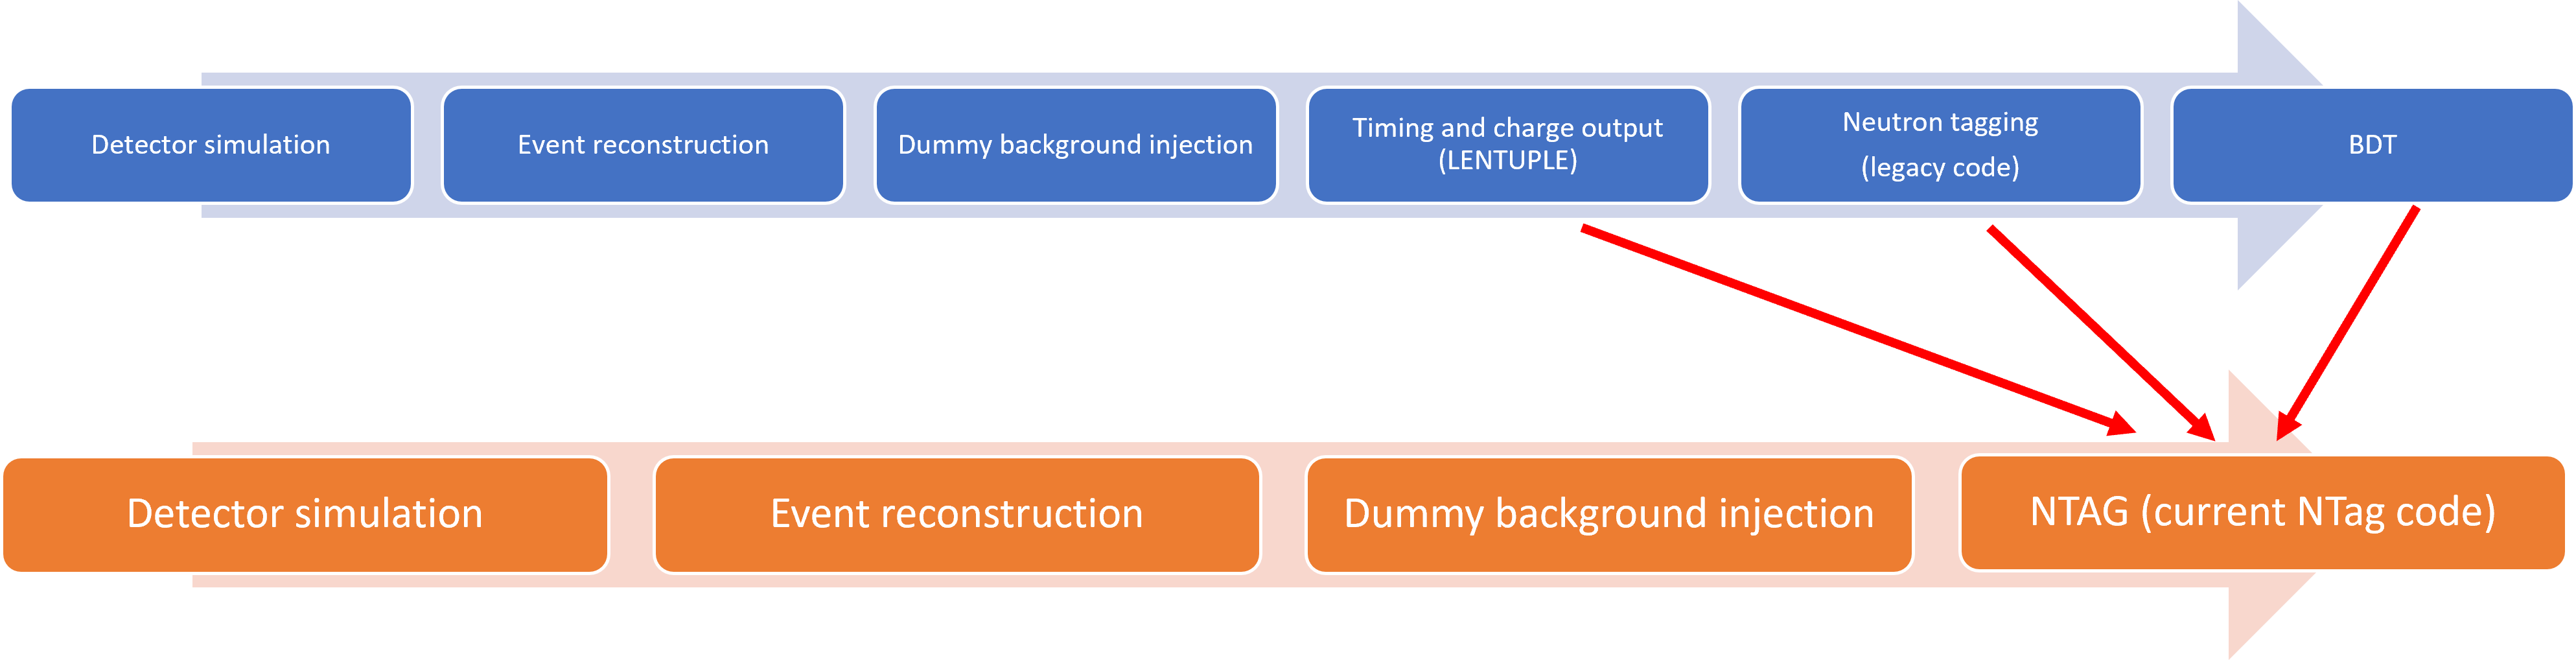
\includegraphics[width=\textwidth]{Figures/analysis_flowchart.png}
    \caption{Flowchart showing the stages in this analysis for both the analysis which used the legacy Ntag code (blue) and the current NTag code (orange).}
\label{fig:analysis_flowchart}
\end{figure}

The main differences between the legacy and new NTag code lie in the neutron tagging algorithm stage, especially regarding variables used to classify the tagged neutron candidates. A large part of this analysis was to ensure that the legacy and new NTag code produced the same results regarding the prompt event and also for the Monte Carlo truth information regarding the neutrons. 



\section{Event Simulation}

This section discusses details about the event simulation, specifically the way neutrino interactions are simulated in order to produce the Monte Carlo. Table \ref{table:software} summarises all the software packages used in this analysis. 


\begin{table}
$$
\begin{array}{ll}
\hline \text { Name } & \text { Version } \\
\hline \text { Flux } & 13 \text { a tuning v4.0 } \\
\text { NEUT } & 5.3 .3 \\
\text { SKDETSIM-SKGd } & \text { ANNRI-Gd model } \\
\text { Geant } & 4.10.05.p01 \\
\text { T2KReWeight } & \text { v1r23 } \\
\text { GENIE } & \text { R2-12-10 } \\
\hline
\end{array}
$$
\caption{Software versions used in analysis from \cite{tn415_fiacob}.}
\label{table:software}
\end{table}

\subsection{Neutrino flux}

 The NA61/SHINE experiment provides hadron production measurements for T2K and other long baseline experiments, and measures the yield of charged hadrons from a proton beam fired at a thin graphite target (2 cm long) and a T2K replica graphite target (90 cm long). From this experimental data, Monte Carlo simulations of the neutrino flux are predicted. In the beam MC, protons which have 30 GeV of kinetic energy are focused onto a graphite target and and after the secondary particles are focused using the horn magnets, the neutrino tracks they decay into are ascertained at the near detectors and at Super-Kamiokande to produce the flux and energy spectra at both of these locations. The oscillation effect on the neutrino flux needs to be considered after choosing which flux to use, and although the neutrino-oxygen NCQE cross section does not depend on flavour (and therefore neutrino oscillation affects would have no impact on a fully pure NCQE sample) there is a small fraction of charged current events which seep into the NCQE sample, and oscillation weights need to be applied to the charged current events in the sample. Monte Carlo reweighting takes care of this issue by assuming that they are all muon neutrino or muon anti-neutrino events, due to the fact that the number of electron neutrino events in FHC mode would be negligible.

\subsection{Primary interaction}

The interaction between the incoming neutrino event and an Oxygen nucleus, and the de-excitation of the nucleus is modelled by NEUT, which produces a vector of primary particles used for event simulaation in SKDETSIM. Because these are primary particles, they do not take into consideration all the particles produced from the detector response, i.e. the secondary particles produced from the interactions within the medium of the detector, in our case, water doped with $\mathrm{Gd}_{2}\left(\mathrm{SO}_{4}\right)_{3} \cdot 8 \mathrm{H}_{2} \mathrm{O}$. The way NEUT treats the interaction between a nucleus and a neutrino for the case of a neutrino interaction with a ${ }^{16} \mathrm{O}$ isotope is shown in Equation \ref{eq:neutrinonuc}. 

\begin{equation}
    \sigma\left(\nu^{16} \mathrm{O}\right)=\sum_{i=1}^{8} \sigma_{\mathrm{p}}\left(p_{i}^{(\mathrm{p})}\right)+\sum_{j=1}^{8} \sigma_{\mathrm{n}}\left(p_{j}^{(\mathrm{n})}\right)+\sigma(2 p 2 h)    
\label{eq:neutrinonuc}    
\end{equation}

Here $\sigma_{p}$ and $\sigma_{n}$ are the neutrino-proton cross section and the neutrino-neutron cross section respectively, and these cross-sections are dependent on the momenta of the protons and neutrons in the model, and therefore on the choice on nuclear model. The Benhar Spectral Function (SF) is used by NEUT as the nuclear model for NCQE interactions, and for CCQE interactions the Smith-Moniz relativistic Fermi Gas (RFG) model is used \cite{benhar_electron-_2005}, with 2p2h interactions included. 

\begin{figure}
    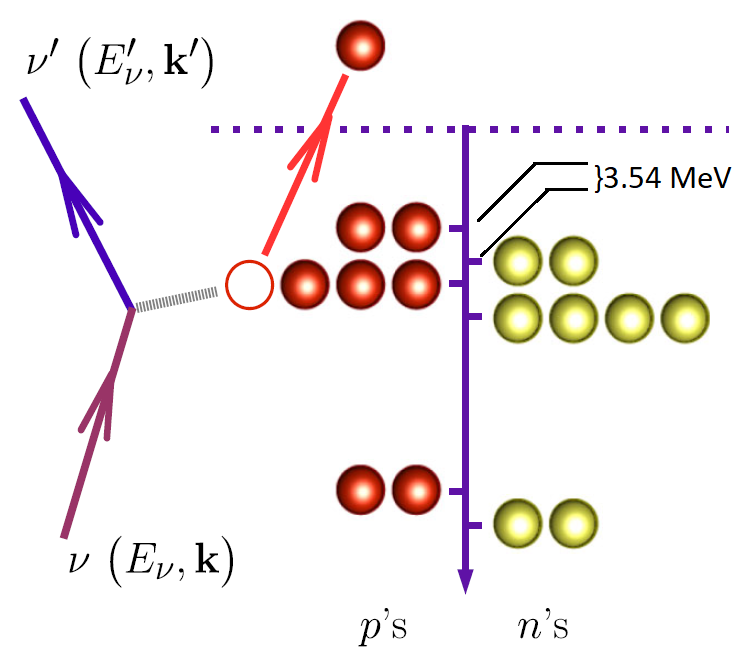
\includegraphics[width=\textwidth]{Figures/ncqebenharspectral.png}
    \caption{Representation of NC neutrino scattering off ${ }^{16} \mathrm{O}$ with protons on the left hand side and neutrons on the right arranged according to the shell model. }
\label{fig:ncqebenharspectral}
\end{figure}

The lowest rung of nucleons in Figure \ref{fig:ncqebenharspectral} is the $s_{1/2}$, with $p_{3/2}$ above this level and $p_{1/2}$ above that. The protons in these rungs have removal energies of 42 MeV, 18.4 MeV and 12.1 MeV respectively, and due to neutron levels being more tightly bound, these have an extra removal of 3.24 MeV compared to their proton counterparts. The shell model is imperfect due to how it allocates the probablity of $16_{O}$ transitioning to the possible nucleon states. In the shell model, probabilities are allocated by counting the number of nucleons in each energy level and assigning probailities according to how many there are. In Figure \ref{fig:ncqebenharspectral} it can be seen that the $p_{3/2}$ state has double the number of nucleons compared to the $s_{1/2}$ model and therefore double the probability of transition is assigned for the $p_{3/2}$ state, and the probability of transitioning to any other state is assigned to be 0, because in the shell model they don't even exist. The Benhar Spectral Function model however is complex and is tuned using electron-nucleus scattering data. The model used in this analysis is a modified version of the Benhar Spectral Function model, where the case of other transition states is dealt with by merging the "others'' state into the $s_{1/2}$ state. Table \ref{table:transitionprob} gives the probabilities of transition to different states for different models. 

\begin{table}
$$
\begin{array}{ccccc}
\hline & \left(\mathrm{s}_{1 / 2}\right)^{-1} & \left(\mathrm{p}_{3 / 2}\right)^{-1} & \left(\mathrm{p}_{1 / 2}\right)^{-1} & \text { others } \\
\hline \text { Shell model } & 0.25 & 0.5 & 0.25 & 0 \\
\text { Spectral Function } & 0.1055 & 0.3515 & 0.158 & 0.385 \\
\text { This analysis } & 0.4905 & 0.3515 & 0.158 & 0 \\
\hline
\end{array}
$$
\caption{Transition probabilities for different models and states}
\label{table:transitionprob}
\end{table}

\subsection{Detector response and interactions in the detector medium}

Prior analyses to this used SKDETSIM (Super-Kamiokande Detector Simulator) to simulate the trajectories of particles through the water in Super-Kamiokande and output detector response MC. This analysis uses SKDETSIM-SKGd to propogate the particles, due to the requirement of needing gadolinium sulphate present in the simulation. The particular isotopes of gadolinium used in the simulation are ${ }^{155} \mathrm{Gd}$ and ${ }^{157} \mathrm{Gd}$ due to their excellent thermal neutron capture cross sections. Table \ref{table:gdtable} shows the relative abundance of various gadolinium isotopes inside natural gadolinium and their associated thermal neutron capture cross sections.

\begin{table}
$$
\begin{array}{rcc}
\hline \text { Isotope } & \text { Abundance }[\%] & \text { Cross-section[b] } \\
\hline{ }^{152} \mathrm{Gd} & 0.200 & 735 \\
{ }^{154} \mathrm{Gd} & 2.18 & 85 \\
{ }^{155} \mathbf{Gd} & \mathbf{1 4 . 8 0} & \mathbf{6 0 9 0 0} \\
{ }^{156} \mathrm{Gd} & 20.47 & 1.8 \\
{ }^{157} \mathbf{Gd} & \mathbf{1 5 . 6 5} & \mathbf{2 5 4 0 0 0} \\
{ }^{158} \mathrm{Gd} & 24.84 & 2.2 \\
{ }^{160} \mathrm{Gd} & 21.86 & 1.4 \\
\hline
\end{array}
$$
\caption{Abundance and thermal neutron capture cross section of various isotopes of Gadolinium}
\label{table:gdtable}
\end{table}

As can be seen in Table \ref{table:gdtable}, not only are ${ }^{155} \mathrm{Gd}$ and ${ }^{157} \mathrm{Gd}$ the most abundant isotopes, they also have extremely high neutron capture cross sections compared to the other isotopes. Equation \ref{eq:gdisotopecaptureeq} shows the neutron capture on both of these isotopes, and the energy of the subsequent gamma rays.

\begin{equation}
\begin{split}
 {n}+{ }^{155} \mathrm{Gd} \rightarrow{ }^{156} \mathrm{Gd}^{*} \rightarrow{ }^{156} \mathrm{Gd}+\gamma  (8.536 MeV)\\
 {n}+{ }^{157} \mathrm{Gd} \rightarrow{ }^{158} \mathrm{Gd}^{*} \rightarrow{ }^{158} \mathrm{Gd}+\gamma  (7.937 MeV)
\end{split}
\label{eq:gdisotopecaptureeq}    
\end{equation}




It is important to therefore model the gamma ray emission spectra from both of these isotopes. The model used by SKDETSIM-SKGd is the ANNRI-Gd model, \cite{10.1093/ptep/ptz002}, \cite{tanaka_gamma_2020}. This uses gamma energy spectrum data from the germanium spectrometer at the ANNRI (Accurate Neutron Nucleus Reaction Measurement Instrument) experiment. This experiment uses the incoming pulsed neutron beam from the Japan Spallation Neutron Source (JSNS) at the Material and Life Science Experimental Facility (MLF) of J-PARC. After a 300 kW beam of protons from the JSNS facility hits a target of mercury and produces neutrons, this neutron beam hits an enriched ${ }^{155} \mathrm{Gd}$ target or a ${ }^{nat} \mathrm{Gd}$ film. The ANNRI spectrometer is placed 21.5 m away from the neutron beam source, with two cluster detectors on either side of the neutron capture target material, which is 13.4 cm away from each cluster detector. Surrounding the target, there are also 8 co-axial germanium detectors. The schematic for the ANNRI-Gd experiment is shown in Figure \ref{fig:annrigd}.

\begin{figure}

        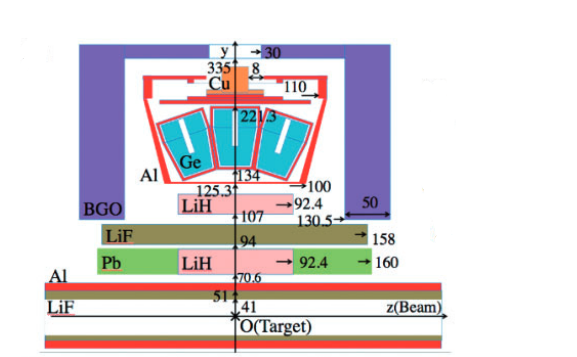
\includegraphics[width=\textwidth]{Figures/annrigd.png}
        \caption{Schematic of the ANNRI Ge spectrometer (dimensions in mm). The beam pipe along with one of the Ge cluster detectors (light blue) is shown. The shaded purple area are the anti-coincidence shields made of bismuth-germanium-oxide (BGO) crystals. \cite{10.1093/ptep/ptz002}.}
        \label{fig:annrigd}
    
\end{figure}

Figure \ref{fig:annrigdenergyspectra} shows the energy spectra for different multiplicity values (left) and hit values (right) from one of the germanium crystals in the ANNRI spectrometer. 

\begin{figure}
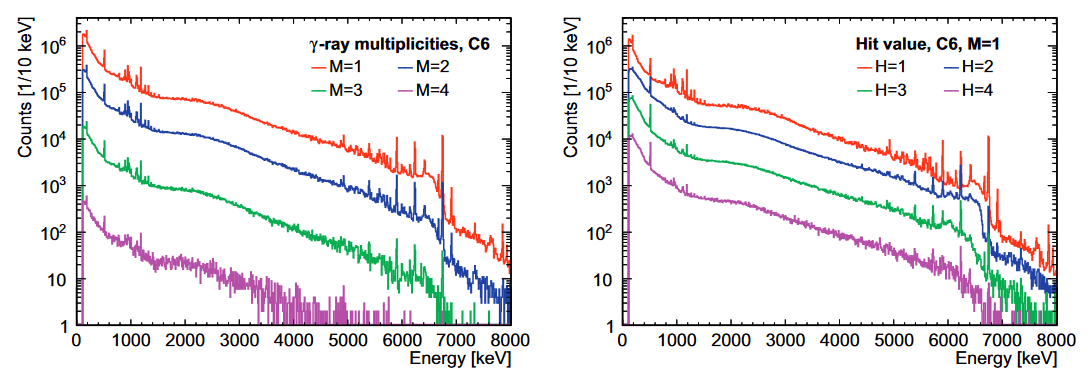
\includegraphics[width=\textwidth]{Figures/annrigdenergyspectra.png}
\caption{Energy spectra for thermal neutron capture on ${ }^{157} \mathrm{Gd}$ energy spectra for different multiplicity values (left) and hit values (right) from one of the germanium crystals in the ANNRI spectrometer.}
\label{fig:annrigdenergyspectra}
\end{figure}

One of the key differences between the default Geant4 model for thermal neutron capture on Gadolinium and the ANNRI-Gd model is how it conserves energy: the photon evaporation model conserves only the final sum of energy for the captured event, but performs poorly when modelling the gamma-ray energy on an individual event by event basis. One way the ANNRI-Gd model combats this is by seperately describing the continuous and discrete peaks in Figure \ref{fig:annrigdenergyspectra}, where the discrete peaks are shown as spikes below 1500 keV and above 4500 keV. These come from the different ways in which gadolinium de-excites after thermal neutron capture. The continuous spectrum in the plots in Figure \ref{fig:annrigdenergyspectra} show the de-excitation of ${ }^{158} \mathrm{Gd}^{*}$ in multiple steps, producing multiple low energy gamma rays, which accounts for about 93\% of the spectrum. The discrete spikes in the spectra come from a two-step cascade, which produces a high energy gamma ray instead, accounting for the remaining 7\% of the spectrum.
Figure \ref{fig:continousdiscrete} shows the continuous and discrete components of the ANNRI-Gd MC, along with data from the experiment. Figure \ref{fig:annrigdmodelcompare} shows ratio plot of data and MC for the GLG4sim model, the default Geant4 photon evaporation model and the ANNRI-Gd model: here it is clear the ANNRI-Gd model fits the data better than the other two models, especially at energies above 3500 keV. The energy from the neutron capture on Gadolinium de-excitation is relased in the form of multiple gamma rays, and liquid scintillator detectors would only have to look for the deposition of the energy from these gamma rays, whereas a water Cherenkov detector such as Super-Kamiokande can only detect part of this deposition due to the Cherenkov threshold energy. As a result, understanding the gamma ray multiplcities and their energies in the range 0.1 MeV to 8 MeV is important in order to predict the efficiency of neutron tagging within Monte Carlo simulation.


\begin{figure}
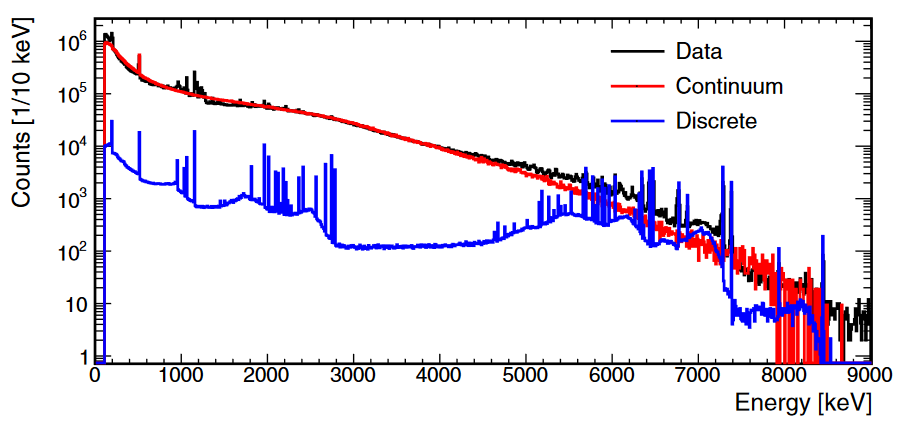
\includegraphics[width=\textwidth]{Figures/continousdiscrete.png}
\caption{Energy spectra for the ANNRI-Gd model broken down into its continous and discrete components along with data from the ANNRI-Gd experiment.\cite{10.1093/ptep/ptz002}}
\label{fig:continousdiscrete}
\end{figure}

\begin{figure}
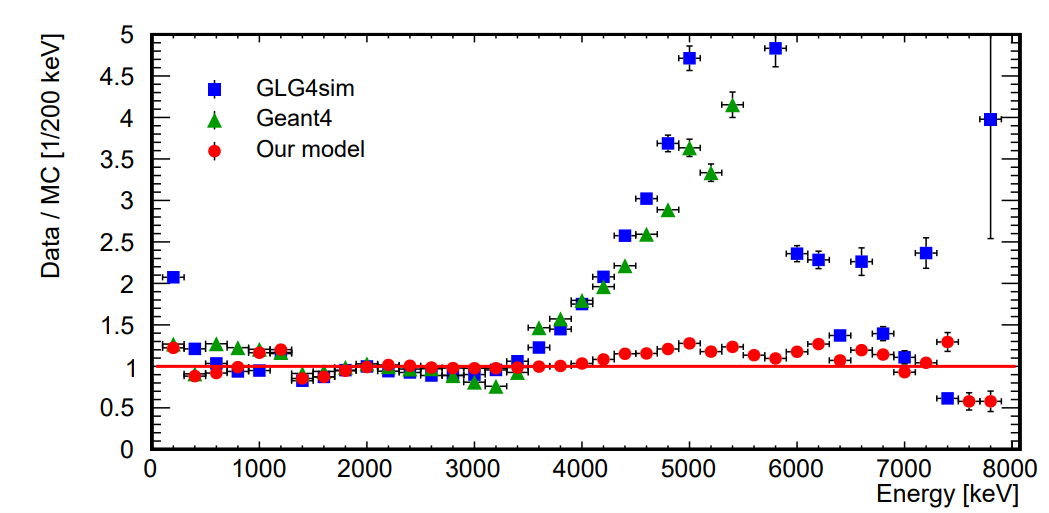
\includegraphics[width=\textwidth]{Figures/annrigdmodelcompare.png}
\caption{Comparison between neutron capture MC models and data, with the ratio of data and MC on the y-axis, the GLG4sim model in blue, Geant4 default model in green and the ANNRI-Gd model in red. \cite{10.1093/ptep/ptz002}}
\label{fig:annrigdmodelcompare}
\end{figure}


\section{Event Reconstruction}
\subsection{Bonsai output reconstruction quantities}

Due to this analysis looking specifically at the low energy region, a fitter specific to low energies (called LOWFIT) is used to reconstruct events. Both MC and data neutrino events undergo a reconstruction phase, where the low-energy fitter BONSAI is applied to the event, as discussed in Chapter 2. The reconstruction is carried out using timing and PMT position information, however charge information is omitted. The output of BONSAI gives information which will be used in the reduction phase of the data and allow for the selection of the NCQE sample. The following quantities comprise the BONSAI output, the first two being helpful spectator variables and the latter five constituting parameters which are used in the reduction phase of the analysis, from which the neutrino NCQE sample is determined.\\


\noindent
\underline{1. Neutrino vertex position}\\
\noindent 
The reconstructed location of the neutrino interaction event.

\noindent
\underline{2. Neutrino vertex direction}\\
\noindent
This vector points towards the direction which is an average over all the Cherenkov cone axes which are produced, due to there being multiple leptons induced in the interaction.


\noindent
\underline{3. Reconstructed energy}\\
\noindent 
In line with the standard SK low energy analysis definition, this energy is simply the reconstructed energy with the 0.511 MeV electron mass omitted. The range for $E_{rec}$ in this variable is 3.49 MeV to 29.49 MeV - the estimated kinetic energy under the hypothesis that the event is a singular electron. The upper value for this range is chosen because the background of Michel electrons (electrons from muon decay) from muon neutrino and muon anti-neutrino charged current interactions increase but the NCQE signal decreases above 30 MeV. 

\noindent
\underline{4. Dwall}\\
\noindent 
This variable gives the minimum distance of the neutrino vertex position from the closest wall of the Super-Kamiokande detector.

\noindent
\underline{5. Effwall}\\
\noindent 
This variable gives the distance between the neutrino vertex position and the closest wall, but moving back from the vertex position along the neutrino vertex direction vector.

\noindent
\underline{6. Vertex direction and goodness coefficient}\\
\noindent 
The coefficient $ovaQ$ (defined in Equation \ref{eq:ovaq}) describes the quality of the vertex reconstruction. It consists of two parameters $g^2_{vtx}$ and $g^2_{dir}$ where the former describes the goodness of the vertex which is based on PMT hit timings, and increases the sharper an event is in time. The latter is the directional goodness and measures the azimuthal uniformity in the ring pattern produced by the Cherenkov cone, which decreases the more uniform an event is in space. As a result of this, $ovaQ$ increases the more uniform and sharp in time an event is.

\begin{equation}
    \text { ova } Q=g_{\text {vtx }}^{2}-g_{\text {dir }}^{2}
    \label{eq:ovaq}
\end{equation}

$g_{vtx}$ is calculated using a fit of the PMT timing distribution and using the hit times of the PMT it is defined as in Equation\ref{eq:vertex_goodness}.

\begin{equation}
g_{\mathrm{vtx}}=\frac{\sum_{i} w_{i} \mathrm{e}^{-\frac{1}{2}(\frac{\Delta t_{i}}{\sigma})^{2}}}{\sum_{i} w_{i}} \text { with } w_{i}=-\frac{1}{2}(\frac{\Delta t_{i}}{\omega})^{2}
\label{eq:vertex_goodness}
\end{equation}

Here $\sum_{i} w_{i}$ is the weight given to the i-th hit PMT for the reduction of dark noise, where $\omega$ has a value of 60ns. $\sigma$ has a value of 5ns which is used to test the goodness, and as a result, a sharp timing distribution produces a large vertex goodness. $g_{dir}$ is calculated by looking at how spatially uniform the hit PMTs are around the reconstructed neutrino vertex direction. In order to quantify this uniformity, the Kolmogorov-Smirnov (KS) test is used as in Equation \ref{direction_goodness}.

\begin{equation}
    \mathrm{g}_{\mathrm{dir}}=\frac{\max _{i}\{\angle_{\mathrm{uni}}(i)-\angle_{\mathrm{data}}(i)\}-\min _{i}\{\angle_{\mathrm{uni}}(i)-\angle_{\mathrm{data}}(i)\}}{2 \pi}
\label{direction_goodness}
\end{equation}

where $\angle_{\mathrm{data}}(i)$ is the azimuthal angle of i-th hit real PMT included in the number of hits in 50ns. $\angle_{\mathrm{uni}}(i)=2 \pi i / N_{50}$ is the azimuthal angle of the i-th virtual PMT hit, but only when uniform distribution of the hits is assumed. As the uniformity of the hit pattern increases, the goodness decreases. 
 


\noindent
\underline{7. Cherenkov angle $\theta_{C}$}\\
\noindent

In order to estimate the Cherenkov opening angle, all the possible combinations of PMT hits of three hit PMTs in a 15 nanosecond timing window are binned. A histogram is produced of these binned angles and divided into 100 bins, and by looking at the seven neighbouring bins with the largest number of entries, peaks in the histogram are located. The middle of the seven bins is chosen to be the Cherenkov angle of the event. Figure \ref{fig:cherenkov_hit_triplet} shows the vertex of the prompt event and three PMT hit vectors which produce the Cherenkov opening angle. 

\begin{figure}
    \centering
    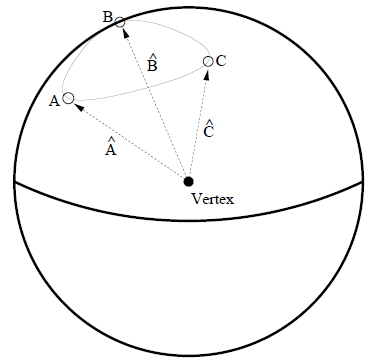
\includegraphics[width=0.7\textwidth]{Figures/cherenkov_hit_triplet.png}
    \caption{Schematic of the prompt event vertex and a triplet of independent PMT hits whch make up the Cherenkov angle}
    \label{fig:cherenkov_hit_triplet}

\end{figure}




 For relativistic electrons in water, the value of the Cherenkov opening angle is $\approx 42\degree$, due to the relation: 

 \begin{equation}
\cos \theta_{\mathrm{Cherenkov}}=\frac{1}{n\beta}
\label{cherenkov_angle}
\end{equation}
 
where $\beta = v/c \approx 1$ and $n$ is the refractive index of water, 1.33. However due to other particles in the simulation, such as protons or muons, the Cherenkov cone is expected to be narrower, or if multiple leptons are present, the Cherenkov cones will be less distinct and more spread out, leading to deviations from the 42\degree value. 

\subsection{Comparison of BONSAI reconstruction output variables between SKDETSIM versions}

The BONSAI reconstruction output variables were compared between three versions of SKDETSIM, the version used in the previous NCQE neutron capture on hydrogen only analysis, with no neutron capture on Gd implemented (black), the SKDETSIM-SKGd photon-evaporation model mentioned in the previous section (red), and the SKDETSIM SK-Gd ANNRI-Gd model (green). Figure \ref{fig:erec_compare} to Figure \ref{fig:thetaC_compare} shows the comparison of these models for the output BONSAI variables $E_{rec}$, dwall, effwall, ovaQ, and $\theta_C$, where the y-axis shows the number of events.

\begin{figure}
    \centering
    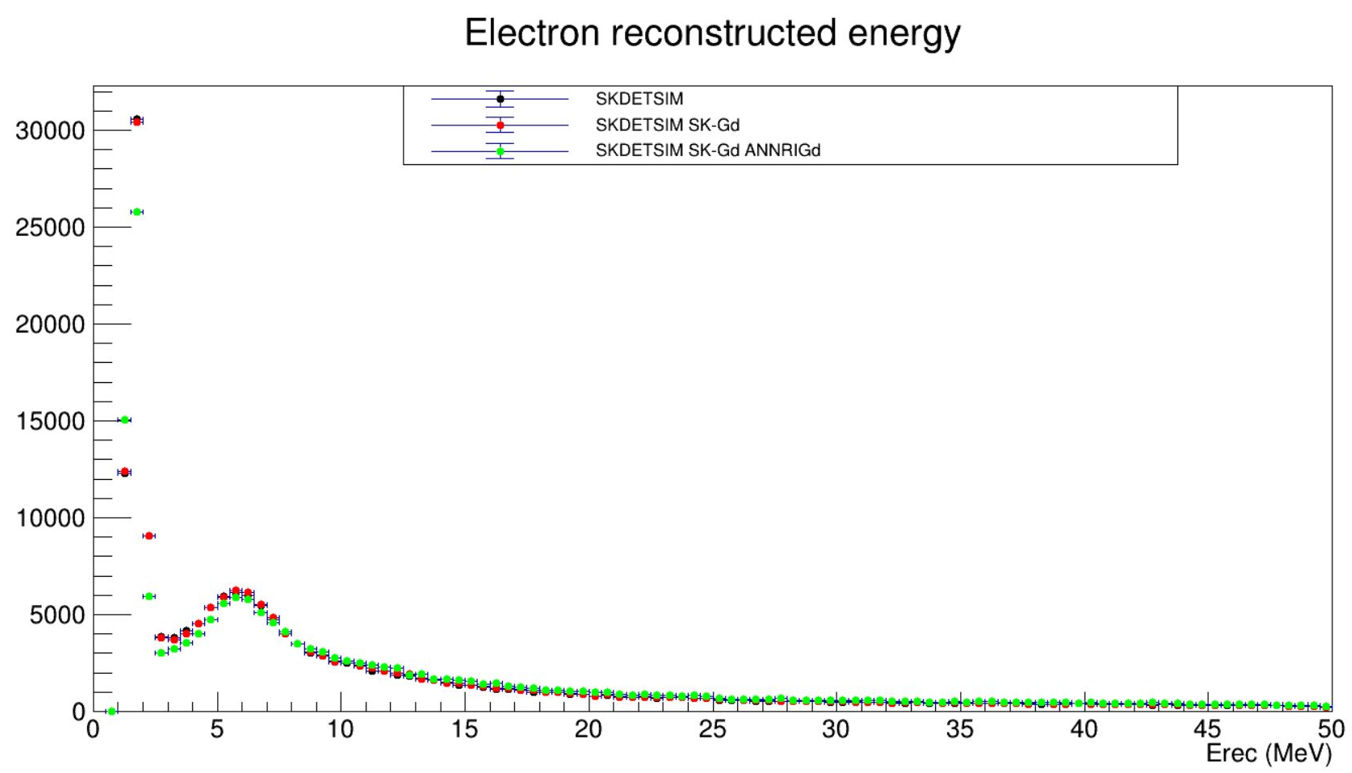
\includegraphics[width=0.7\textwidth]{Figures/erec_compare.png}
    \caption{Comparisons of prompt event electron reconstructed energy between versions of SKDETSIM}
    \label{fig:erec_compare}

\end{figure}

\begin{figure}
    \centering
    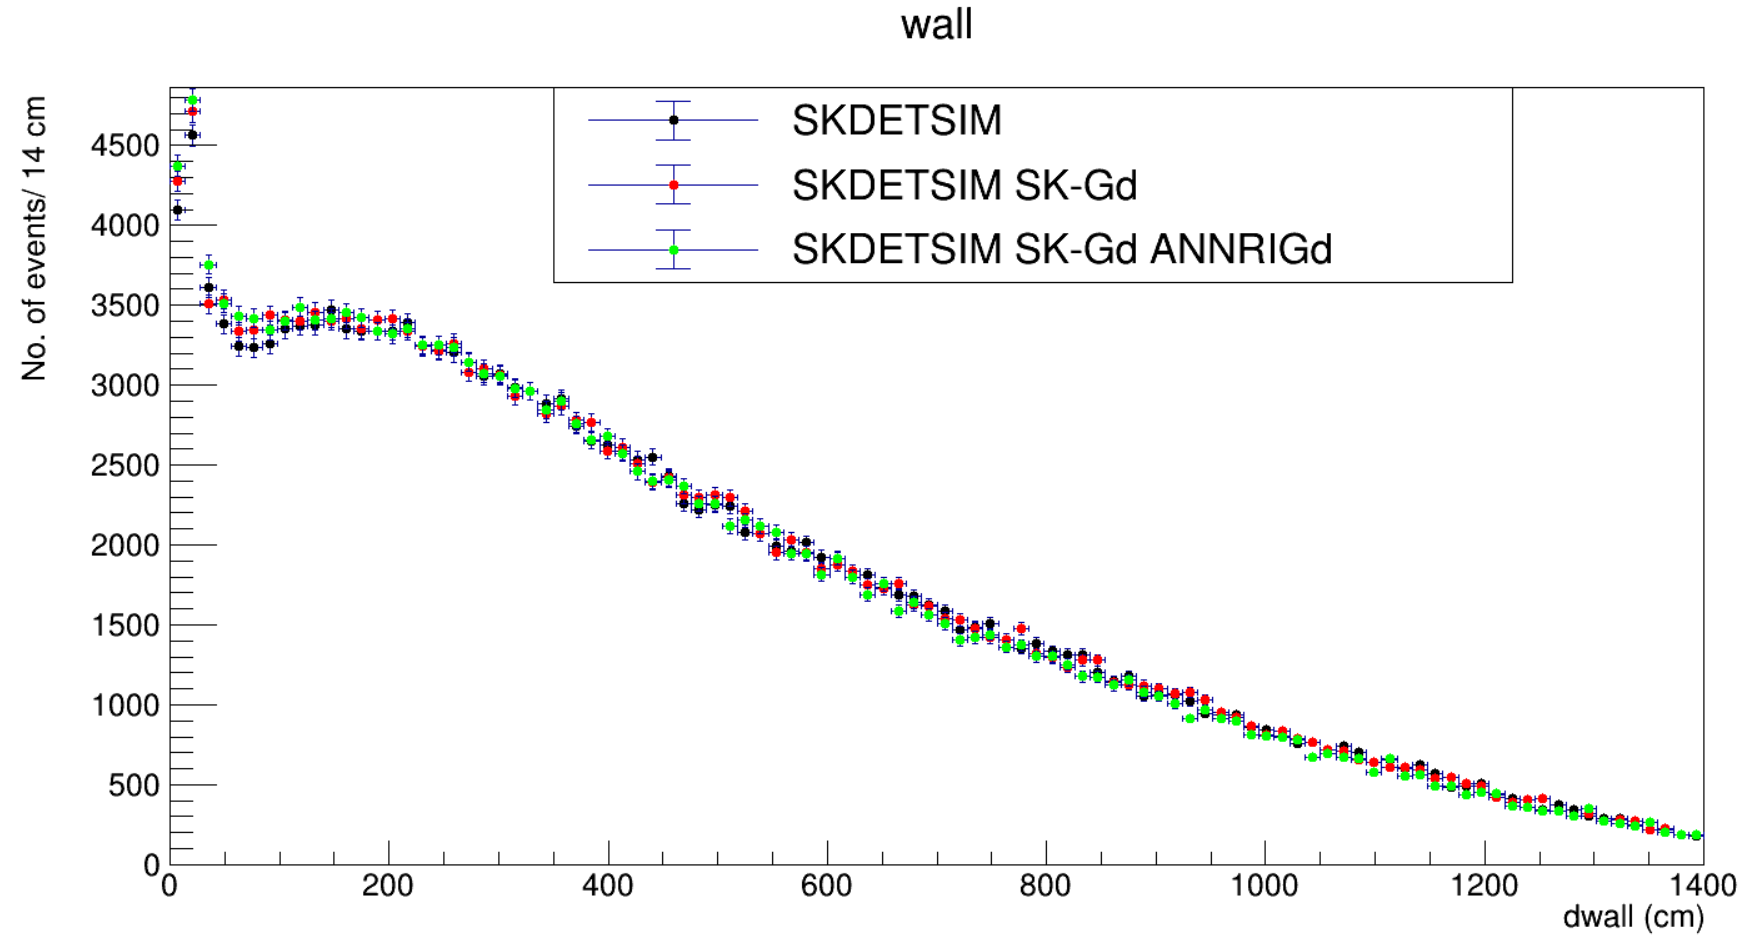
\includegraphics[width=0.7\textwidth]{Figures/dwall_compare.png}
    \caption{Comparisons of dwall for the prompt event between versions of SKDETSIM}
    \label{fig:dwall_compare}

\end{figure}

\begin{figure}
    \centering
    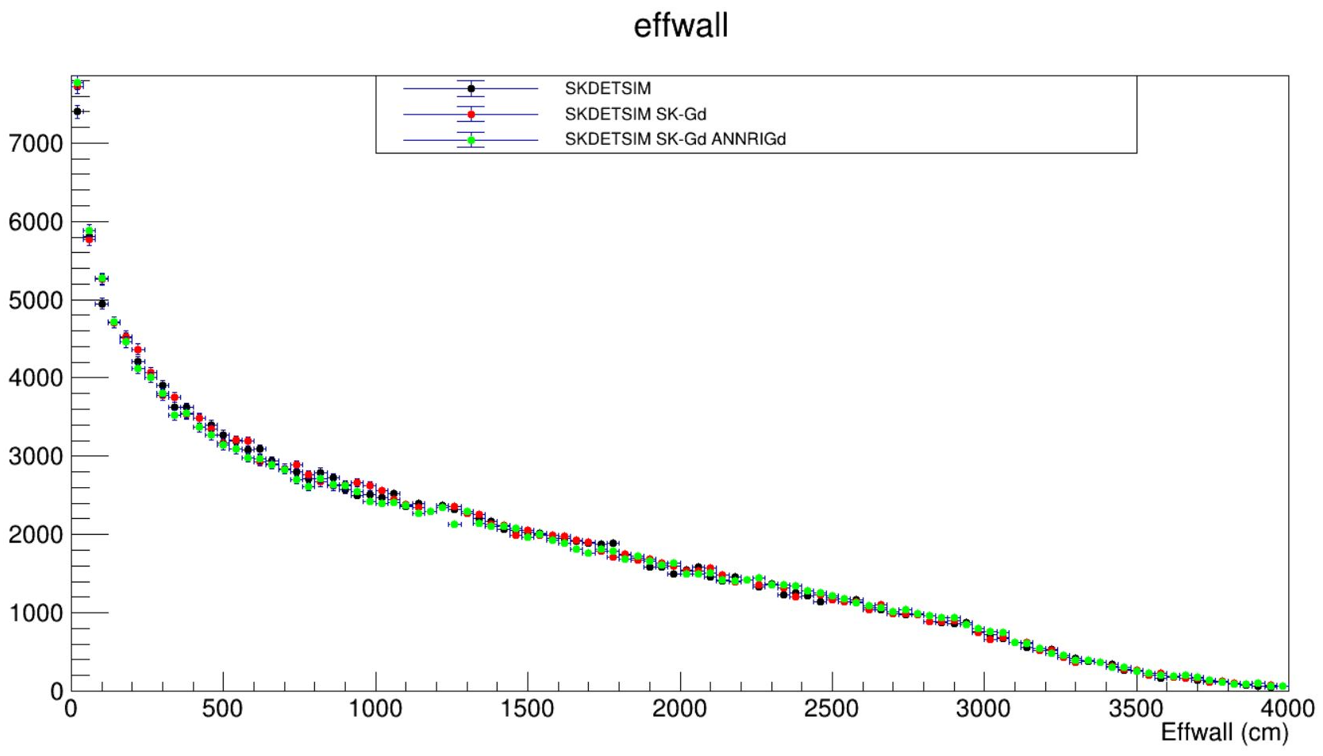
\includegraphics[width=0.7\textwidth]{Figures/effwall_compare.png}
    \caption{Comparisons of effwall for the prompt event between versions of SKDETSIM}
    \label{fig:effwall_compare}

\end{figure}

\begin{figure}
    \centering
    \includegraphics[width=0.7\textwidth]{Figures/ovaQ_compare.png}
    \caption{Comparisons of ovaQ for the prompt event between versions of SKDETSIM }
    \label{fig:ovaQ_compare}

\end{figure}

\begin{figure}
    \centering
    \includegraphics[width=0.7\textwidth]{Figures/thetaC_compare.png}
    \caption{Comparisons of Cherenkov angle for the prompt event between versions of SKDETSIM}
    \label{fig:thetaC_compare}

\end{figure}

\begin{figure}
    \centering
    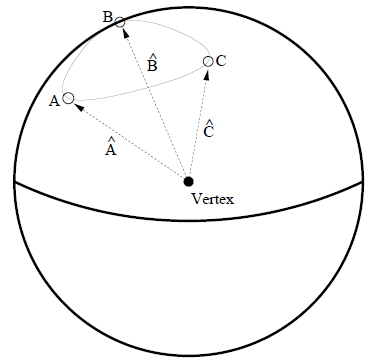
\includegraphics[width=0.7\textwidth]{Figures/cherenkov_hit_triplet.png}
    \caption{Schematic of the prompt event vertex and a triplet of independent PMT hits whch make up the Cherenkov angle}
    \label{fig:cherenkov_hit_triplet}

\end{figure}

To ensure correct implementation of the ANNRI-Gd model, ensuring the BONSAI output variables were similar between these SKDETSIM versions was important as the Gadolinium model should only effect the neutron capture in the simulation, not the output from event reconstruction of the neutrino interaction vertex. As can be seen in Figure \ref{fig:bonsai_reconstruction_compare}, this holds true for $E_{rec}$, dwall, effwall and $\theta_C$, but not for the vertex and goodness coefficient ovaQ, where the ANNRI-Gd model differs for ovaQ between -0.05 and 0.15 compared to the SKDETSIM and SKDETSIM photon-evaporation model. To investigate this difference further, distributions of the vertex goodness and the directional goodness which make up ovaQ (according to Equation \ref{eq:ovaq}) were also checked, shown in Figure \ref{fig:ovaq_compare}.



\begin{figure}
    \centering
    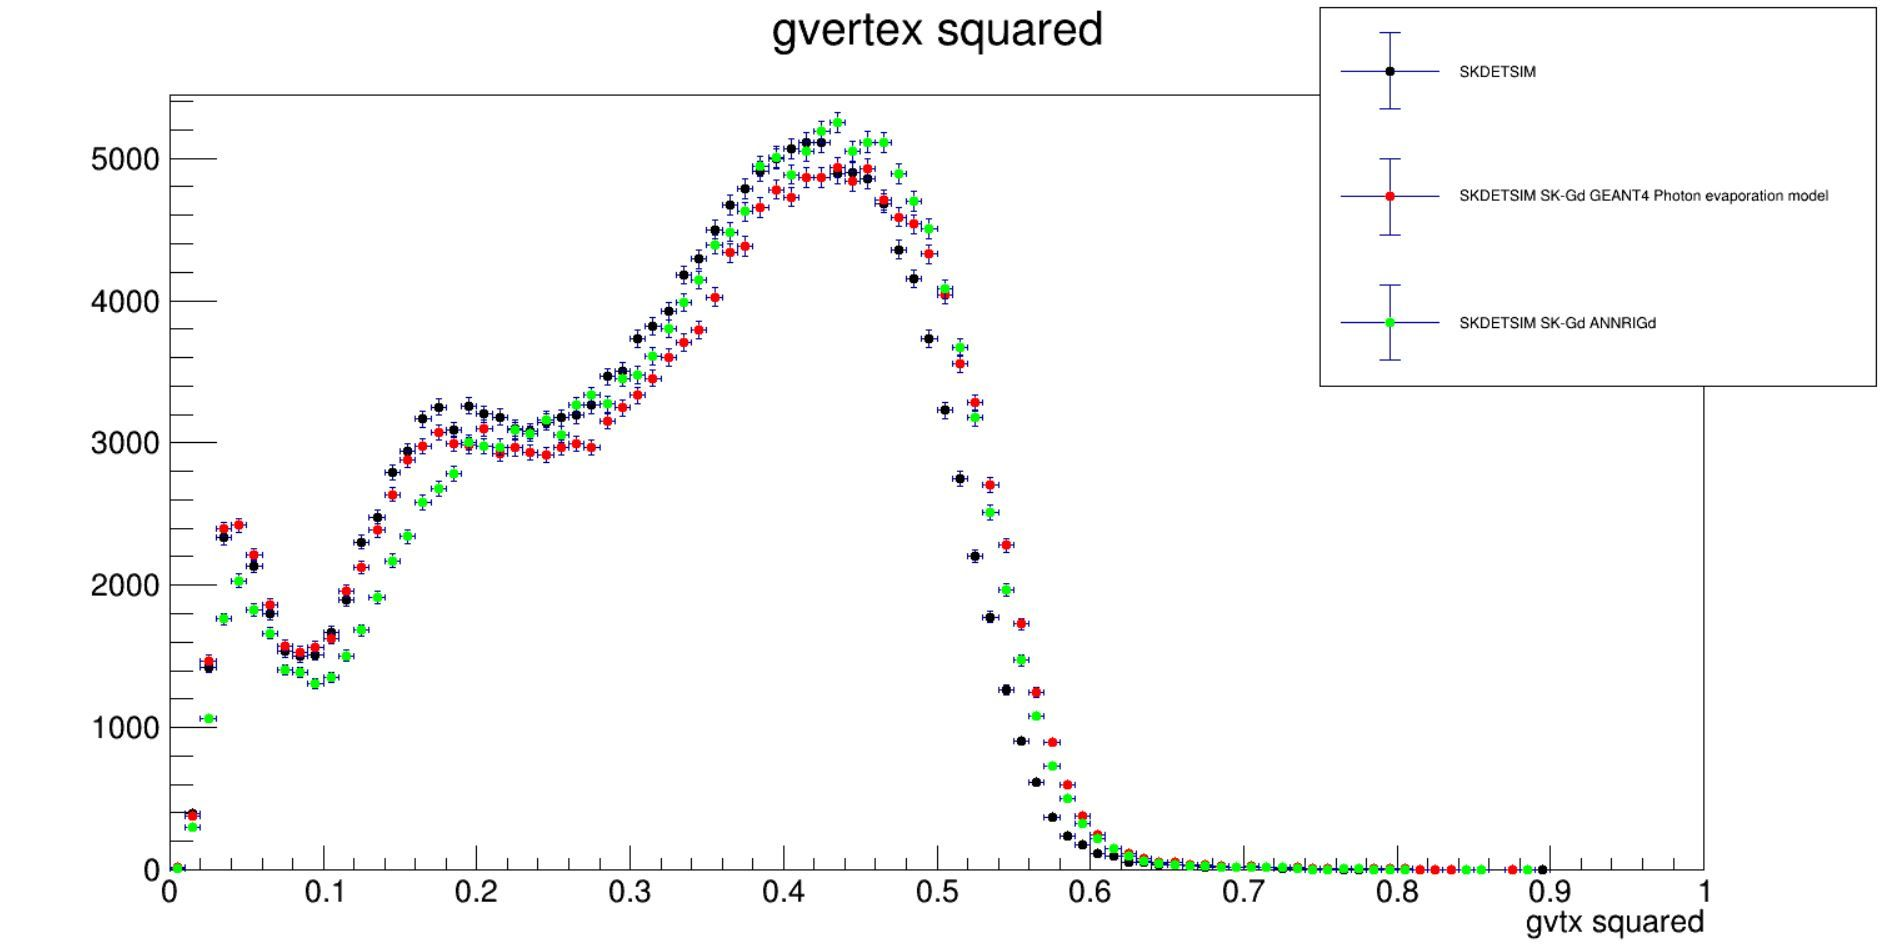
\includegraphics[width=0.7\textwidth]{Figures/gvtx_squared.jpeg}
    \caption{Comparisons of vertex goodness for the prompt event between versions of SKDETSIM}
    \label{fig:gvtx_squared}

\end{figure}

\begin{figure}
    \centering
    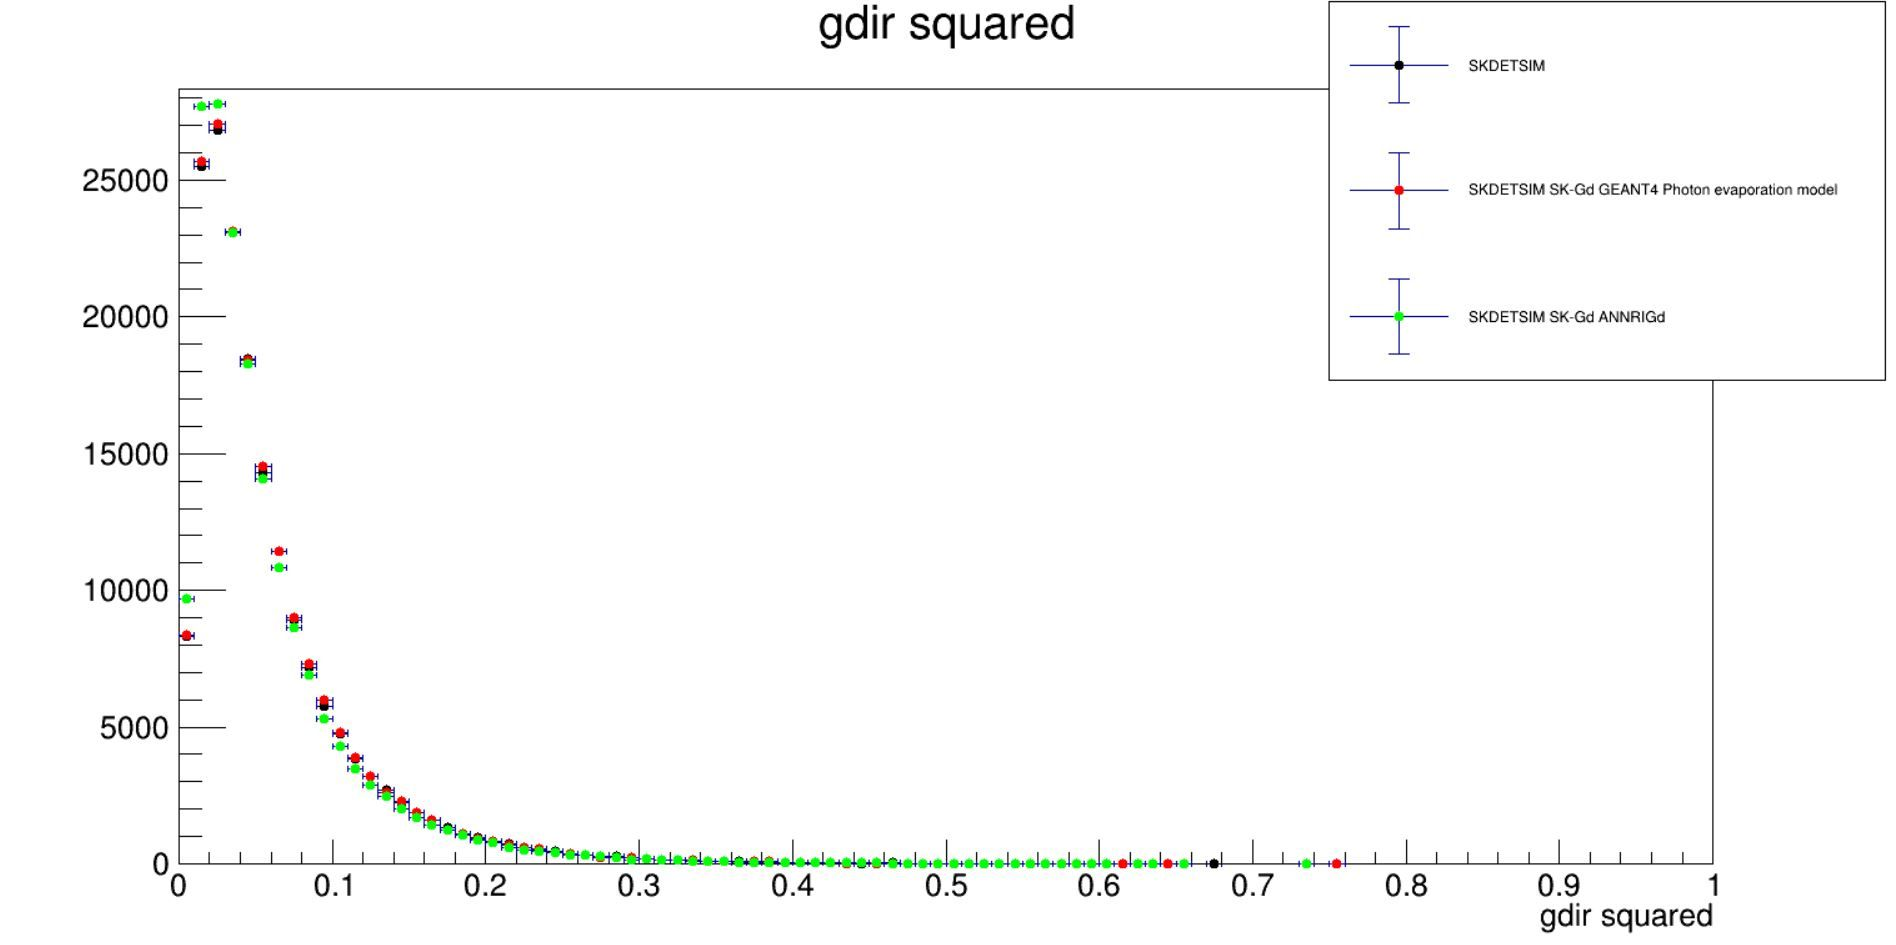
\includegraphics[width=0.7\textwidth]{Figures/gdir_squared.jpeg}
    \caption{Comparisons of directional goodness for the prompt event between versions of SKDETSIM}
    \label{fig:gdir_squared}

\end{figure}

The vertex goodness (gvtx) and directional goodness (gdir) squared comparisons are shown in Figures \ref{fig:gvtx_squared} and \ref{fig:gdir_squared} respectively. Figure \ref{fig:gvtx_squared} shows a slight discrepancy between the SKDETSIM versions, but not enough to warrant further investigation. In addition to checking the previous BONSAI reduction phase quantities, the distance between the true neutrino vertex from the simulation and the neutrino vertex from the BONSAI reconstruction was also checked for the different SKDETSIM versions, shown in Figure \ref{fig:vertex_resolution}. Table \ref{table:vertex_resolution} shows the value of this distribution which encompasses 1-sigma (68\%) of the number of events: this value was very similar for all SKDETSIM versions.
\begin{figure}

    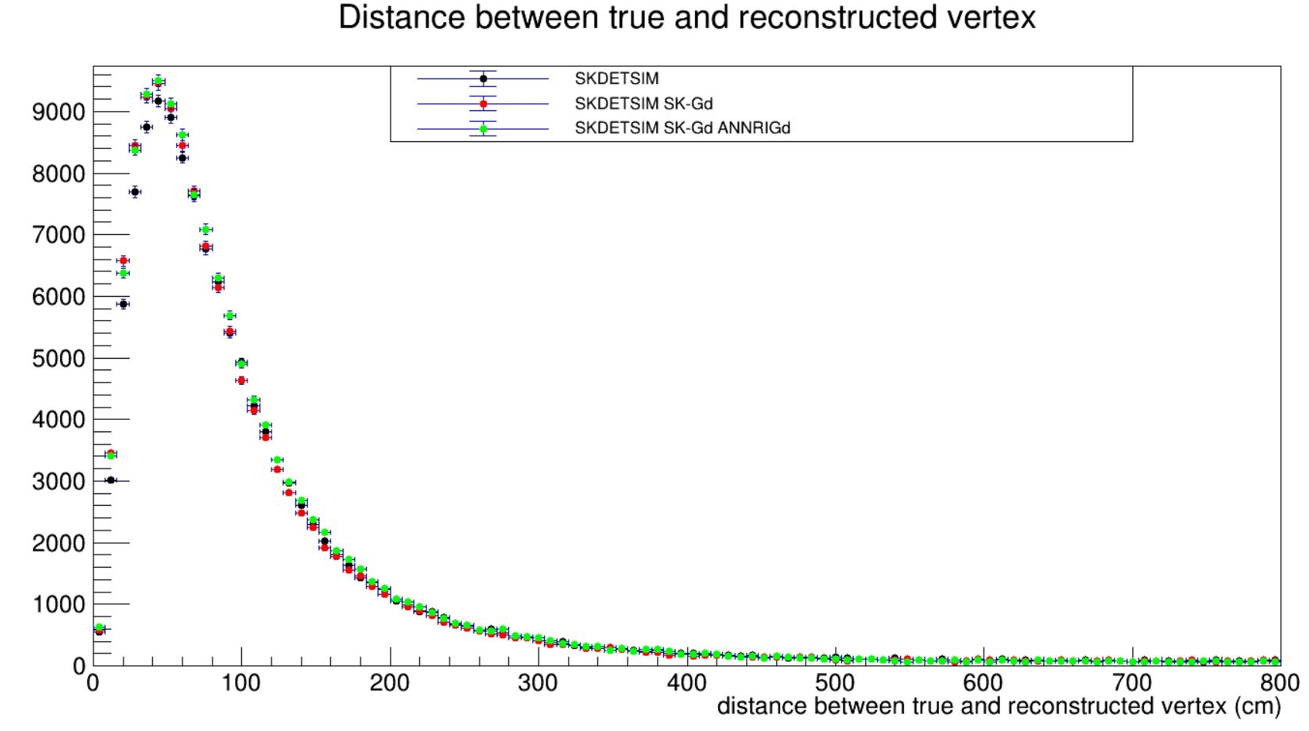
\includegraphics[width=\textwidth]{Figures/vertex_resolution.png}
    \caption{Distance between true and reconstructed neutrino vertex for different SKDETSIM versions}
    \label{fig:vertex_resolution}

\end{figure}

\begin{table}
    $$
    \begin{array}{rcc}
    \hline \text { SKDETSIM version } & \text{Value (cm)} \\
    \text{SKDETSIM-V} & 113.2\\
    \text{SKDETSIM-SKGd (Photon evaporation model)} & 109.4 \\
    \text{SKDETSIM-SKGd (ANNRI-Gd model)} & 111.9 \\
    \hline
    \end{array}
    $$
\caption{Value of the true neutrino vertex - reconstructed neutrino vertex distribution which encompasses 1-sigma (68\%) of the number of events.}
\label{table:vertex_resolution}
\end{table}

\subsubsection{Comparisons of event reconstruction output between NTag versions}
To ensure that the NCQE event selection and neutron tagging could be carried out using the new NTag code, comparisons of the output BONSAI reconstruction variables between the two versions were made to ensure the validity of the reconstruction output. Figure \ref{fig:bonsai_output_compare} shows the reconstructed energy, dwall, effwall, Cherenkov angle and ovaQ parameters, with the legacy NTag output in black and the new NTag output in red. 


\begin{figure}
        \centering
        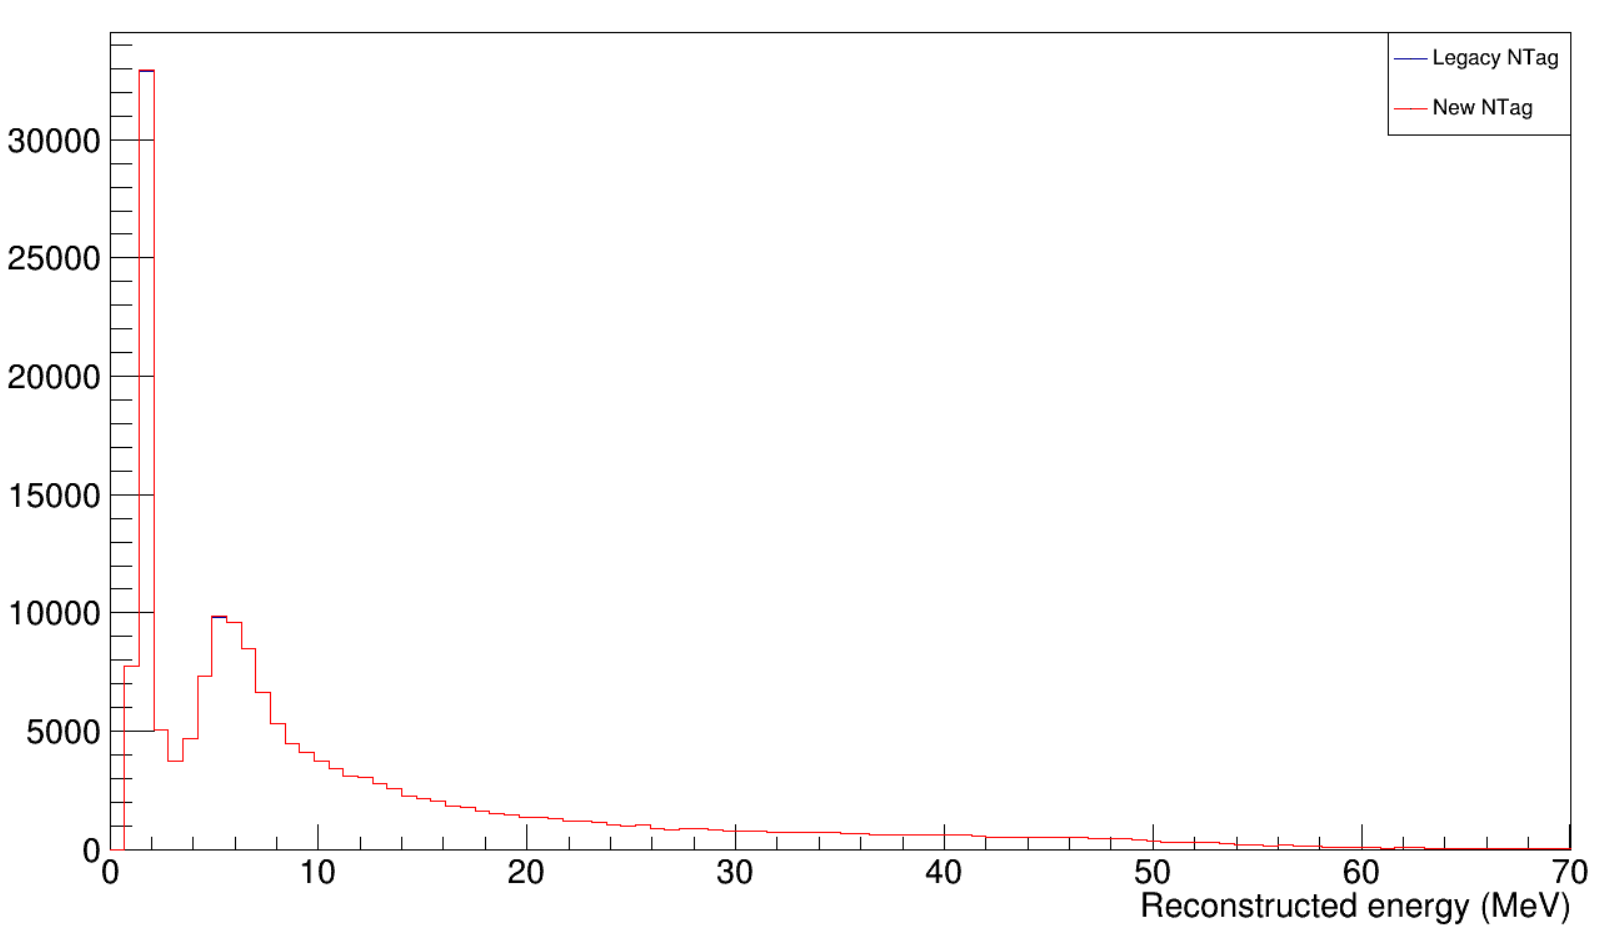
\includegraphics[width=0.9\textwidth]{Figures/energy_recon_compare.PNG}
        \caption{Reconstructed energy (MeV) comparison}
        \label{fig:gvtx_squared}    
\end{figure}

\begin{figure}
    \centering
    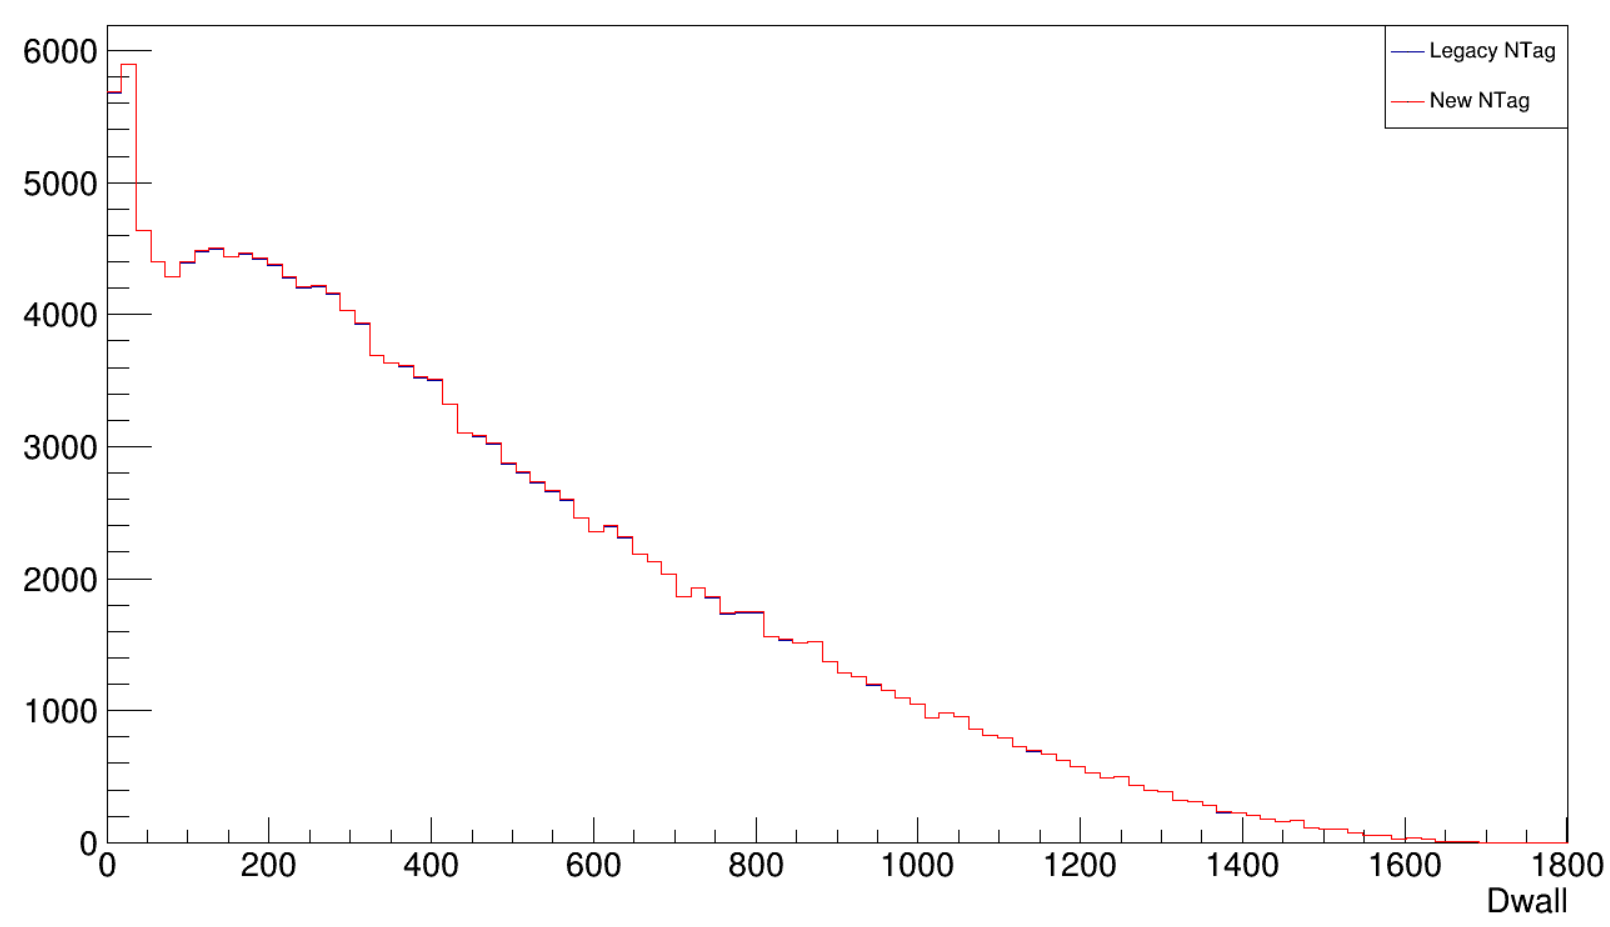
\includegraphics[width=0.9\textwidth]{Figures/dwall_recon_compare.PNG}
    \caption{DWall (cm) comparison}
    \label{fig:gvtx_squared}

\end{figure}

\begin{figure}
    \centering
    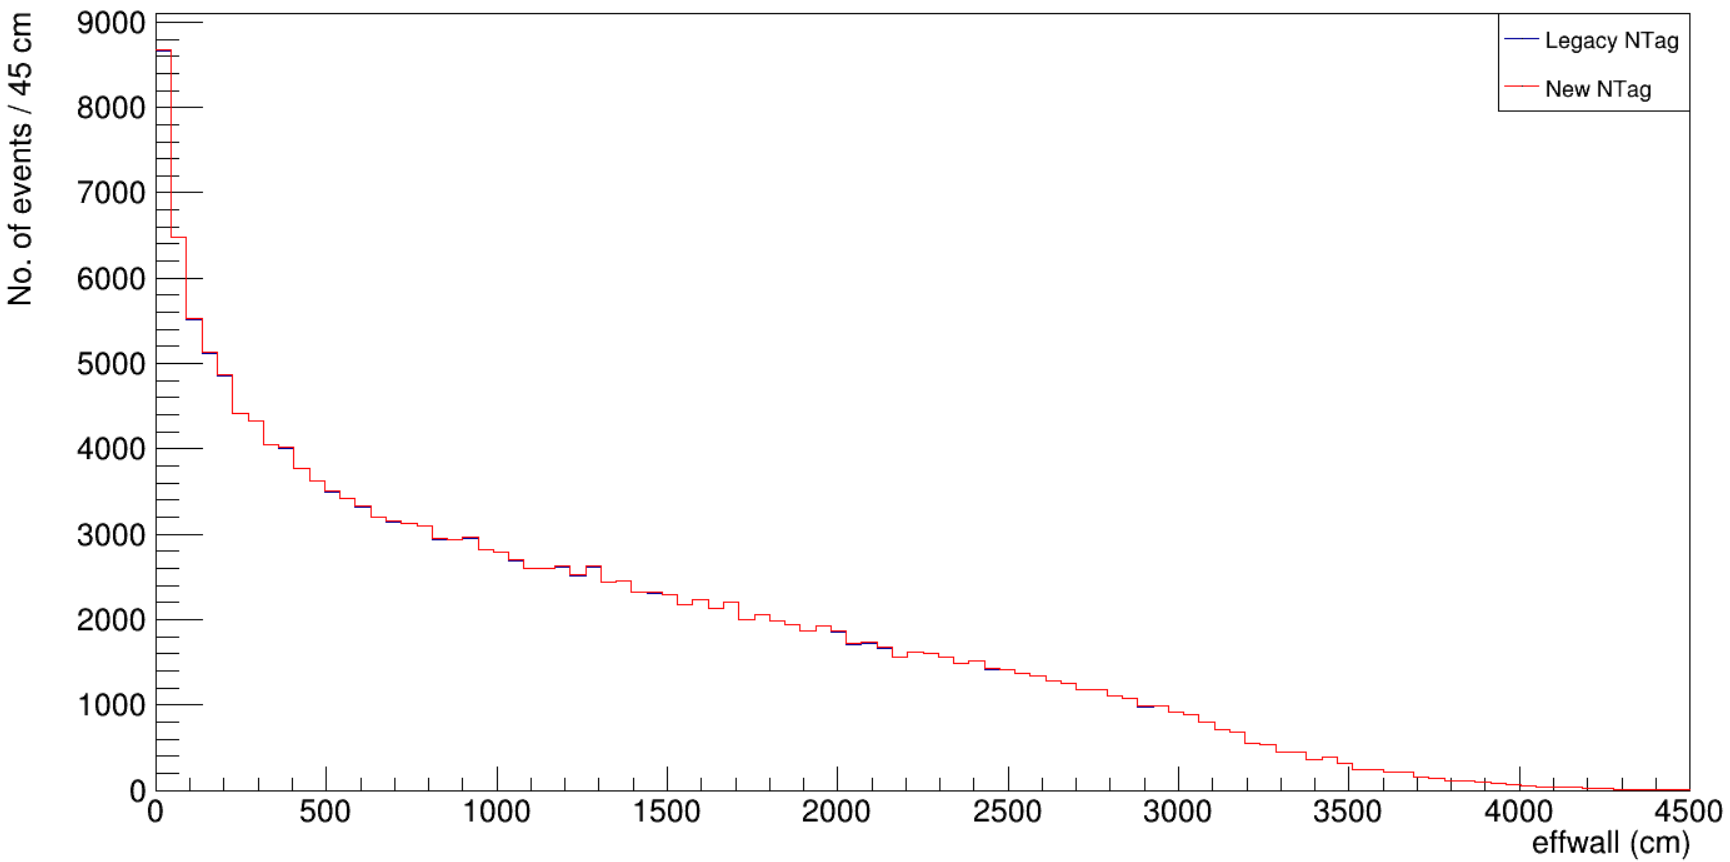
\includegraphics[width=0.9\textwidth]{Figures/effwall_recon_compare.PNG}
    \caption{Effwall (cm) comparison}
    \label{fig:gvtx_squared}

\end{figure}

\begin{figure}
    \centering
    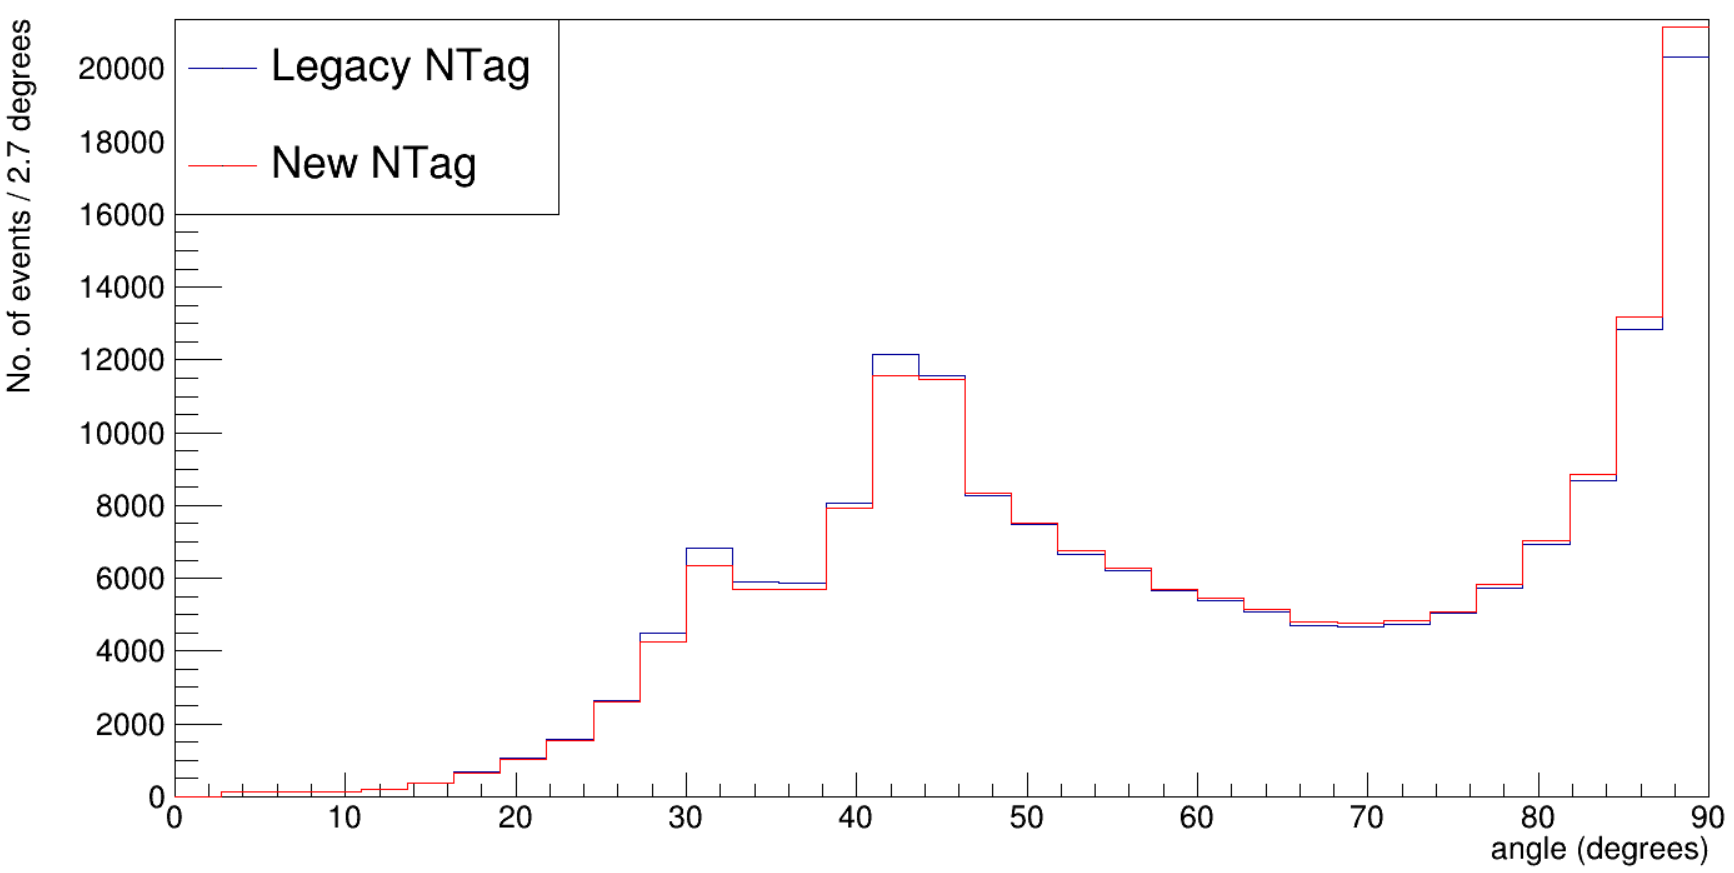
\includegraphics[width=0.9\textwidth]{Figures/angle_recon_compare.PNG}
    \caption{OvaQ comparison}
    \label{fig:gvtx_squared}

\end{figure}

\begin{figure}
    \centering
    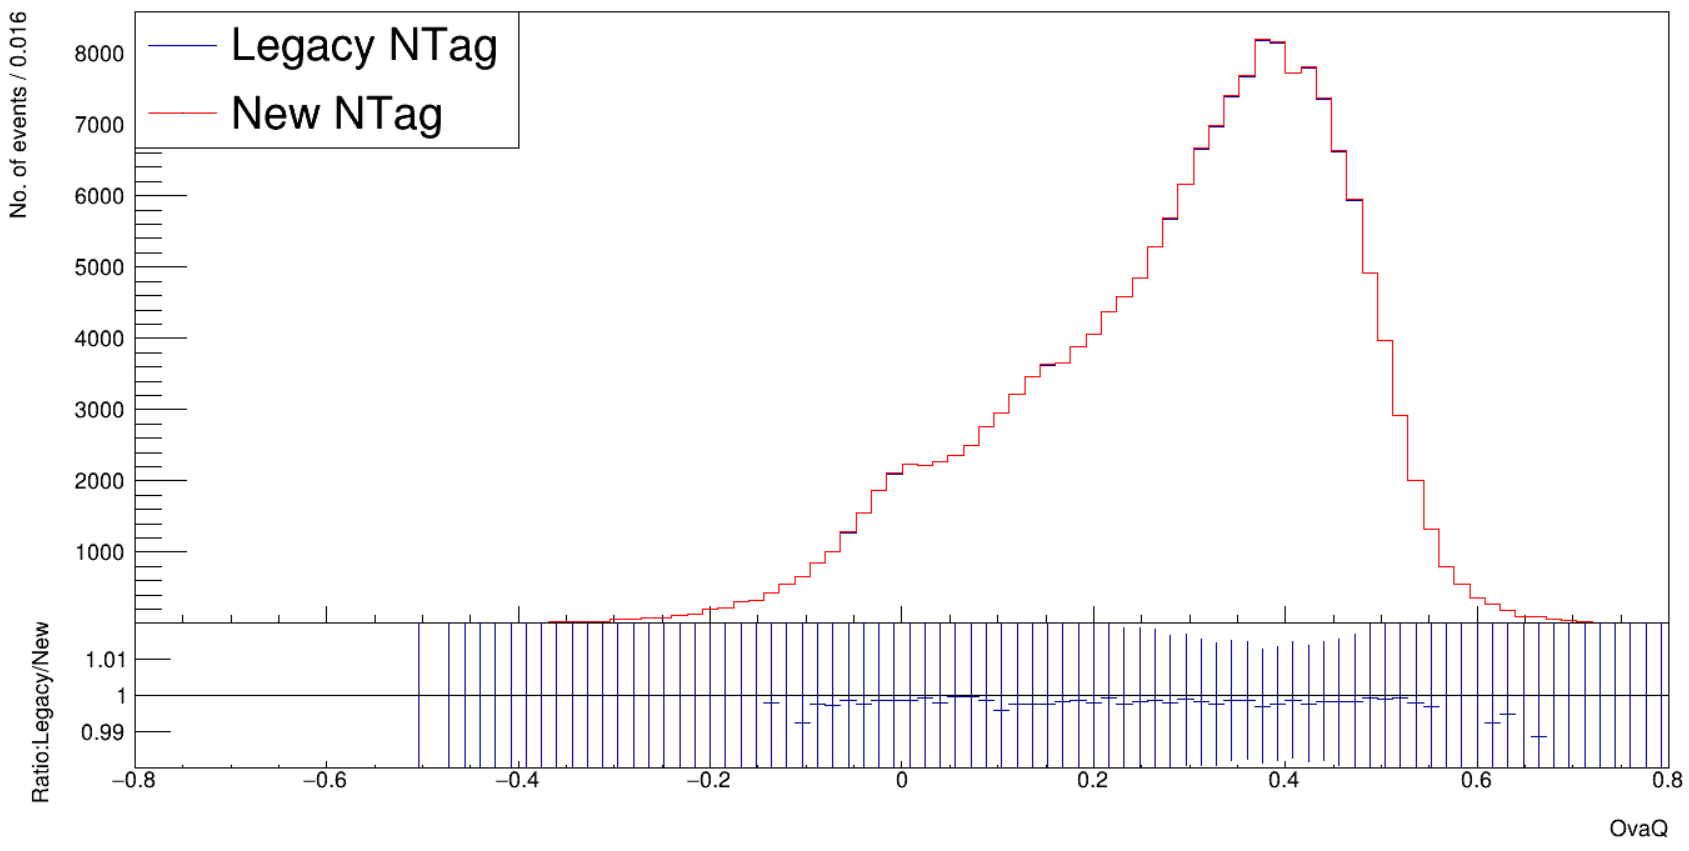
\includegraphics[width=0.9\textwidth]{Figures/ovaq_recon_compare.PNG}
    \caption{Comparisons of vertex goodness for the prompt event between versions of SKDETSIM}
    \label{fig:gvtx_squared}

\end{figure}

From the comparisons of the event reconstruction variables we can conclude that there is no significant variation between the way the different gadolinium implentation models in the detector simulation doesn't affect the way the prompt event is reconstructed. This makes sense as the only difference the neutron capture model should make should relate to the secondary interactions - checking the prompt event distributions remain unchanged is a confirmation of this. Similarly, the comparisons between the two NTag versions, legacy and new show that the change in the neutron tagging algorithm didn't affect the prompt event reconstruction either. 


\subsection{NCQE event selection}

Prior to applying the neutron tagging algorithm which searches for neutron candidates, events which satisfy the neutral current quasi-elastic criteria need to be selected. This selection only involves the neutrino vertex information, no information about the neutron candidates is used in the NCQE selection process. 
\newline
The following cuts are applied to the Monte Carlo, in order to select the NCQE events. These include a visible energy cut, a fiducial volume cut, a low energy background cut, and a cut to exclude charged currrent interaction events (CCQE). 

\subsubsection{Visible energy cut}
The energy window for this analysis is set to the 3.49-29.49 MeV range, where the lower value of this range (3.49 MeV) is due to the detection threshold of Super-Kamiokande. In order to limit the background of the Michel electron from charged-current interactions involving muon neutrinos and muon anti-neutrinos, the upper energy window limit is set to 29.49 MeV - above this value the Michel electron background would increase, reducing the NCQE contribution. 

\subsubsection{Fiducial Volume (FV) cut}
Due to radioactive impurities inside the detector material, specifically the wall of the inner detector, there is a cut involving the distance from the detector wall to the prompt interaction vertex. Events where the distance between the prompt interaction vertex and the detector wall is less than 200 cm are removed. There is a similar cut also used where events where the distance between the prompt interaction vertex and the distance to the inner detector wall in the neutrino vertex vector direction is less than 200 cm is removed. This is a standard cut applied in all Super-Kamiokande analyses in order to avoid backgrounds, and when you have events where the energy region is below 6 MeV even more stringent cuts are required to further reduce background from the inner detector wall, described in the next Subsection. 

\subsubsection{Low energy background cut}

The variables dwall, effwall and ovaQ are used to tune cuts in the energy region below 6 MeV. There are five energy regions with a width of 0.5 MeV used between the lower end of the visible energy cut region (3.49 MeV) and 5.99 MeV where the cuts on the dwall, effwall and ovaQ variables are optimised. Cuts are applied on the dwall, effwall and ovaQ variables and an event is only accepted if the values of dwall, effwall and ovaQ are greater than the threshold cut values. In each 0.5 MeV energy interval, these threshold values are optimised based on the T2K run period due to the beam power and detector conditions being different from run to run, especially since the Gadolinium loading occured in the detector. Equation \ref{eq:FOM} shows how the figure-of-merit (FOM) value is to be maximised for the optimsation of each cut.

\begin{equation}
    \mathrm{FOM}=\frac{N_{\text {sig }}}{\sqrt{N_{\text {sig }}+N_{\text {bkg }}}} \quad\left(N_{\text {bkg }}=N_{\text {bkg }}^{\mathrm{MC}}+N_{\text {bkg }}^{\text {beam-unrelated }}\right)
\label{eq:FOM}
\end{equation}

Here $N_{sig}$ is the number of NCQE neutrino events in the FHC Monte Carlo sample and $N_{bkg}$ is the summation of the background events, and the FOM is calculated seperately in the five energy intervals, and the optimised cut value is taken as the one which maximises the FOM. Then the optimised cut values in each energy interval are fitted with a linear function dependent on the visible energy variables ($E_{rec}$). Equation \ref{eq:FOM_linear} gives the relation of $E_{rec}$ to the optimised cut values for dwall, effwall and ovaQ.

\begin{align}
    \text { dwall }^{\text {CUT }} =p_{0}^{\text {dwall }}+p_{1}^{\text {dwall }} \times E_{\text {rec }} \\
    \text { effwall }^{\text {CUT }}=p_{0}^{\text {effall }}+p_{1}^{\text {effwall }} \times E_{\text {rec }} \\
    \text { ova } Q^{C U T}=p_{0}^{\text {ovaQ }}+p_{1}^{\text {ovaQ }} \times E_{\text {rec }}
\label{eq:FOM_linear}
\end{align}


The scan regions and intervals for the dwall, effwall and ovaQ parameters for Equation \ref{eq:FOM_linear} are given in \cite{Abe_2019}. 

\subsection{Charged current event (CC) interaction cut}

In order to reduce the number of charged-current events which may be mistakenly included in the NCQE selection, a cut regarding the reconstructed Cherenkov angle of the prompt event  is also utilised alongside the low energy background cut, where the accepted Cherenkov angle of a prompt event ($theta_{C}$) should be greater than the threshold cut value $\theta_{C}^{CUT}$ where the cut value is determined by the linear equation dependent on $E_{rec}$ as shown in Equation \ref{eq:thetaC_FOM}.

\begin{equation}
    \theta_{C}^{C U T}=p_{0}^{\theta_{C}}+p_{1}^{\theta_{C}} \times E_{\text {rec }}
    \label{eq:thetaC_FOM} 
\end{equation}

Just like for the low energy background cut values, the values of the optimised parameters in Equation \ref{eq:thetaC_FOM} are given in \cite{Abe_2019}.


\subsection{Prompt event NCQE reduction cut plots}

Before applying the NTag algorithm, either legacy or new, plots were produced of the number of neutrino events and their dependence the reduction cut variables mentioned previously. These are shown in Figures \ref{fig:erec_reduction}, \ref{fig:dwall_reduction}, \ref{fig:effwall_reduction}, \ \ref{fig:ovaq_reduction}, \ref{fig:angle_reduction}. Each figure shows the corresponding plot for the previous NCQE analysis carried out with neutron tagging on Hydrogen on the left, with the plot from this analysis on the right. 


\begin{figure}[!htbp]
    \centering
    
    \caption{Comparisons of stacked histrograms for the $E_{rec}$ variable between NCQE neutron tag on H analysis (left) and this analysis (right)} \label{fig:erec_reduction} 
    
    \subfloat[]{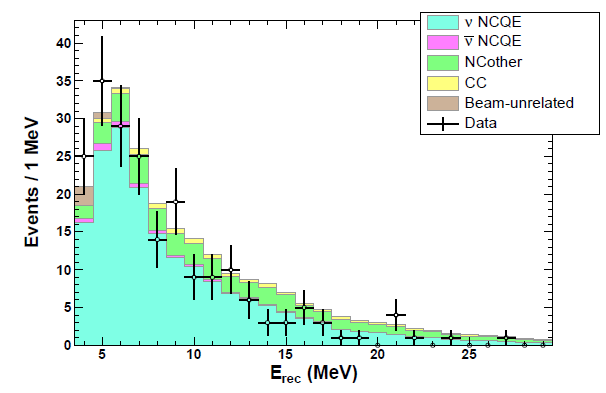
\includegraphics[width=0.49\textwidth]{Figures/fabio_erec.PNG}}  \hfill 
    \subfloat[]{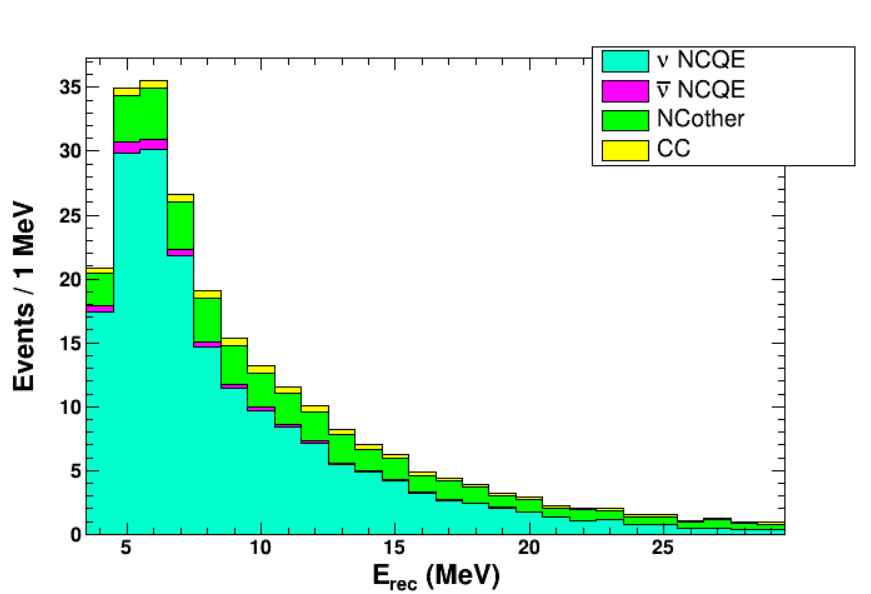
\includegraphics[width=0.49\textwidth]{Figures/erec_reduction.PNG}} \par
    
        
\end{figure}

\begin{figure}[!htbp]
    \centering
    
    \caption{Comparisons of stacked histrograms for the Dwall variable between NCQE neutron tag on H analysis (left) and this analysis (right)} \label{fig:dwall_reduction} 
    
    \subfloat[]{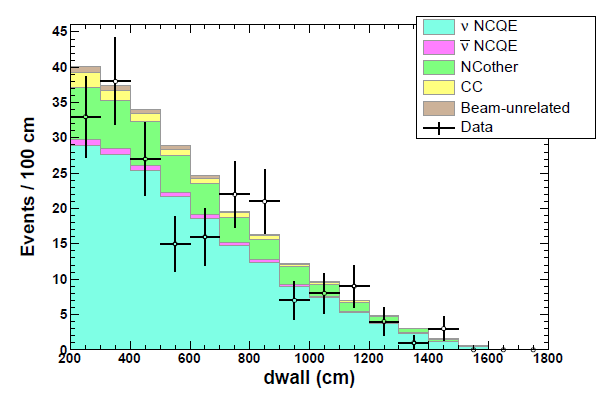
\includegraphics[width=0.49\textwidth]{Figures/fabio_dwall.PNG}}  \hfill 
    \subfloat[]{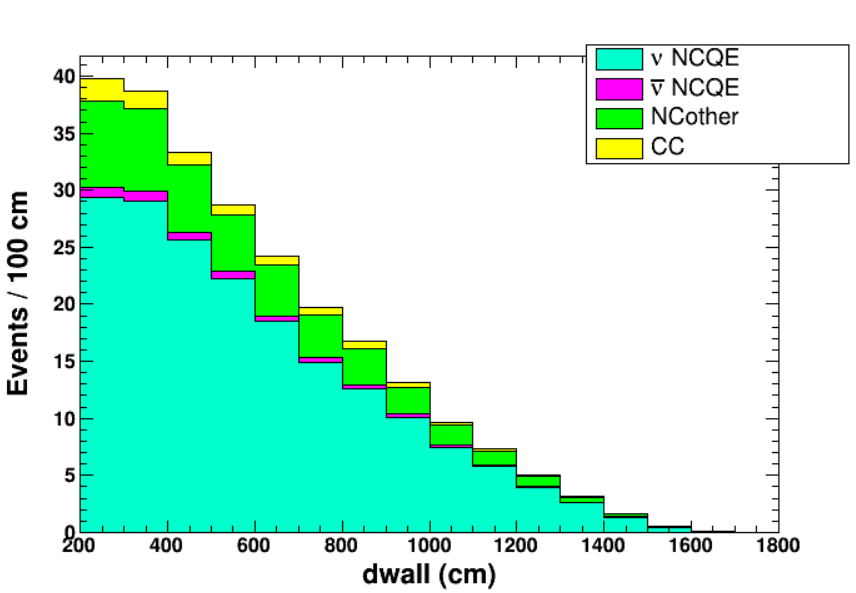
\includegraphics[width=0.49\textwidth, height=4.2cm]{Figures/dwall_reduction.PNG}}  \par
    
        
\end{figure}

\begin{figure}[!htbp]
    \centering
    
    \caption{Comparisons of stacked histrograms for the Effwall variable between NCQE neutron tag on H analysis (left) and this analysis (right)} \label{fig:effwall_reduction} 
    
    \subfloat[]{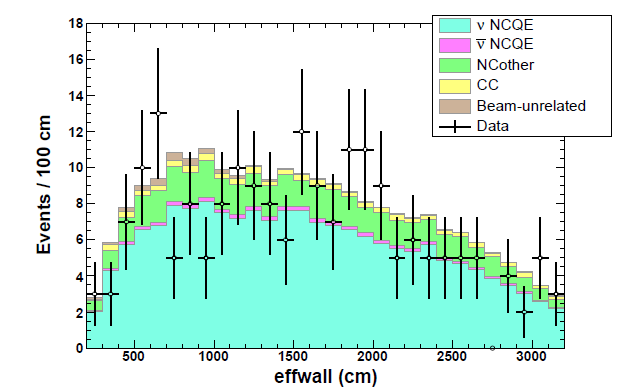
\includegraphics[width=0.49\textwidth]{Figures/fabio_effwall.PNG}}  \hfill 
    \subfloat[]{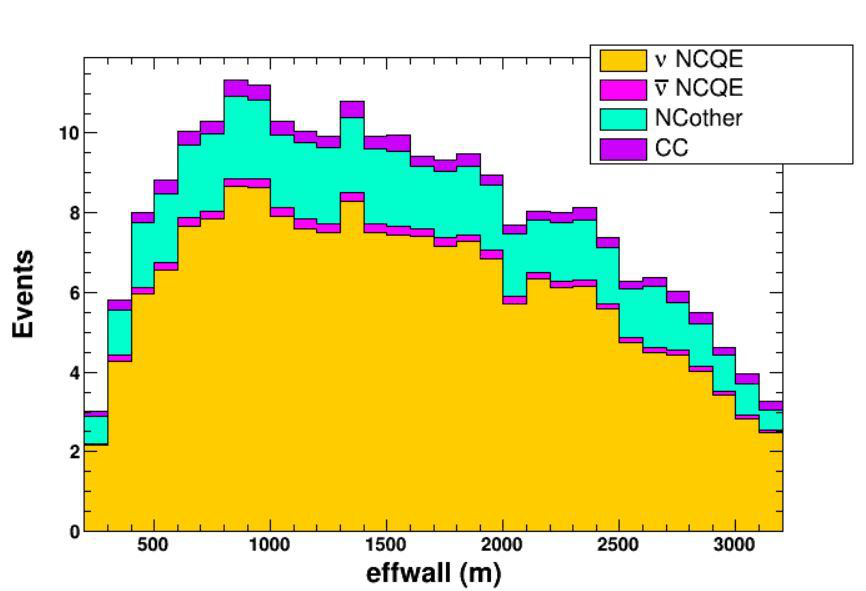
\includegraphics[width=0.49\textwidth]{Figures/effwall_reduction.PNG}} \par
    
        
\end{figure}

\begin{figure}[!htbp]
    \centering
    
    \caption{Comparisons of stacked histrograms for the ovaQ variable between NCQE neutron tag on H analysis (left) and this analysis (right)} \label{fig:ovaq_reduction} 
    
    \subfloat[]{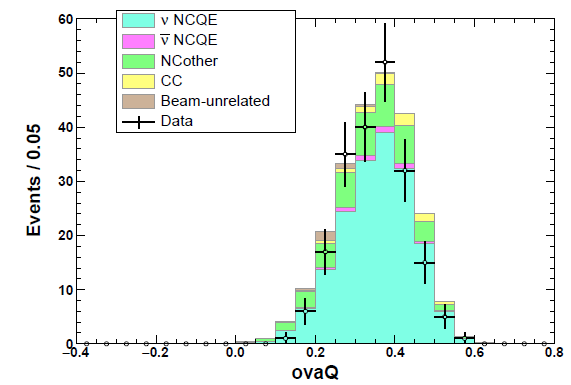
\includegraphics[width=0.49\textwidth]{Figures/fabio_ovaq.PNG}} \hfill 
    \subfloat[]{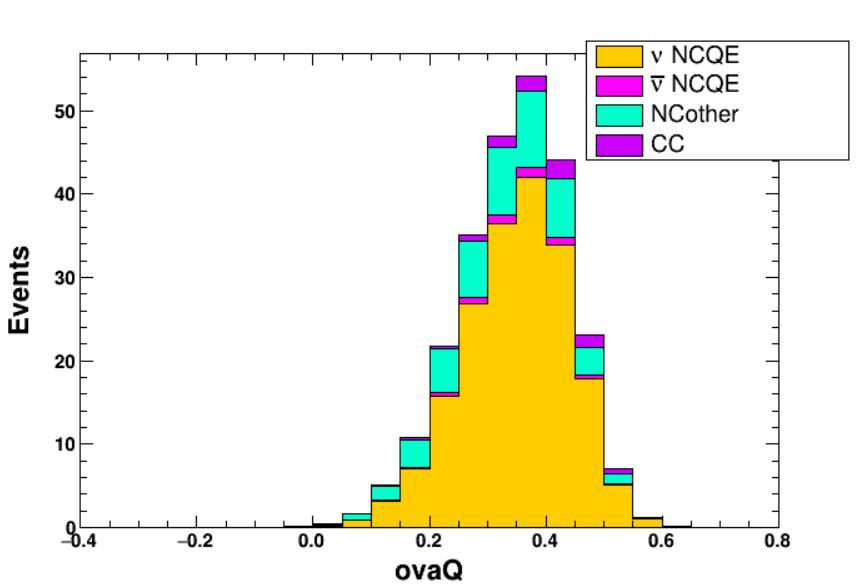
\includegraphics[width=0.49\textwidth]{Figures/ovaq_reduction.PNG}} \par
    
        
\end{figure}

\begin{figure}[!htbp]
    \centering
    
    \caption{Comparisons of stacked histograms for the $\theta_C$ variable between NCQE neutron tag on H analysis (left) and this analysis (right)} \label{fig:angle_reduction} 
    
    \subfloat[]{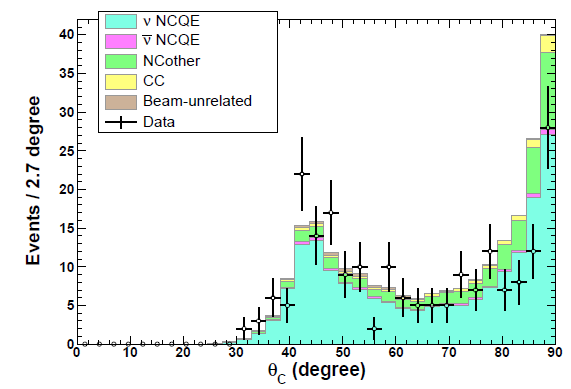
\includegraphics[width=0.49\textwidth]{Figures/fabio_angle.PNG}} \hfill 
    \subfloat[]{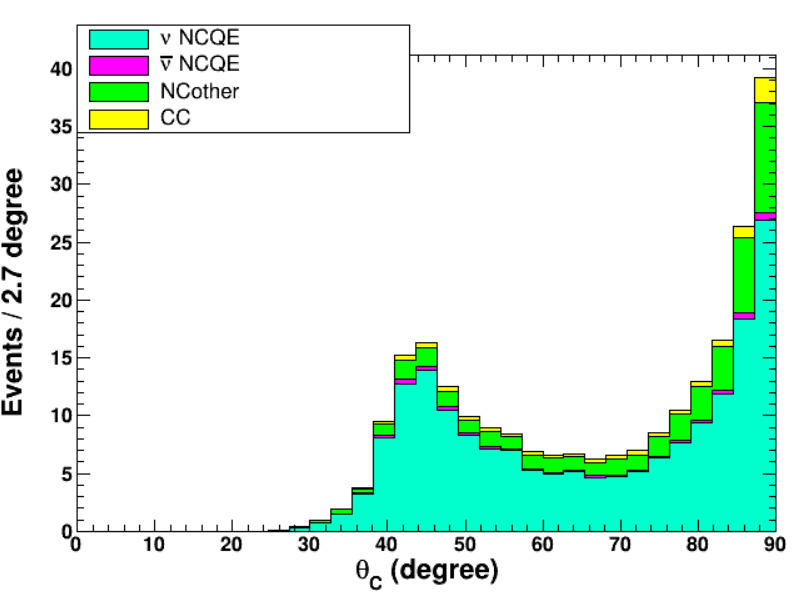
\includegraphics[width=0.49\textwidth, height=4.2cm ]{Figures/angle_reduction.PNG}} \par
    
        
\end{figure}

\subsection{Background injection}

Low energy backgrounds play a big role in this analysis because of the captures on neutrons including neutron capture on Hydrogen producing a 2.2 MeV energy signal. The two main sources of background in this analysis come from environmental radioactvity and PMT dark noise. The signal hits are mixed in with the dark noise hits and stem from the PMTs themselves, with no dependence on individual PMTs meaning that the distribution of dark noise in the detector is expected to be uniform. A Poisson distribution represents the dark noise for the PMTs in the detector, and therefore the mean value of dark noise hits $<\#DN>$ in a time window of $T$ nanoseconds for the total number of inner detector PMTs, $N_{ID}$, where the dark noise rate of one PMT averaged over an entire inner detector is $<dark>$ is given in Equation \ref{eq:dark_noise_hits}. 



\begin{equation}
        \begin{aligned}
        \langle \# D N \rangle &=\langle\text { dark }\rangle \times T \times N_{I D} \\
        &=10.0 \frac{\mathrm{kHz}}{\mathrm{PMT}} \times 14 \mathrm{nsec} \times 11,146 \mathrm{PMT}=1.56
        \end{aligned}
        \label{eq:dark_noise_hits} 
\end{equation}

The previous NCQE analysis with solely neutron capture occuring on Hydrogen used a $T$ = 10 nsec timing window for the neutron capture search (the criteria for which will be detailed in the next section) and a $<dark>$ rate of 5.0 kHz per PMT. However since the addition of gadolinium sulphate octahydrate in the detector medium, the dark rate per PMT has doubled and to accomadate for neutron captures occuring on the gadolinium the neutron capture hit search window has been increased to 14 nsec. 

The dark noise hits from natural radioactivity comes from unstable isotopes from the detector material, PMT covers, the Tyvek lining the tank and the rock from the cavern which Super-Kamiokande resides in. These decaying unstable isotopes can produce enough hits to produce a signal that looks like a neutron capture on Hydrogen, meaning that these hits from natural radioactvity could also get mixed in with the hits in the 14 nsec neutron search timing window. Simulating this combination of dark noise and radioactivity in the tagged neutron candidate search window is not trivial, and therefore it is far easier to inject actual background data into the neutron search window. This background data is collected in the form of ``dummy spills'' which are events which are taken during periods where the T2K beam is switched off, i.e. events in between T2K runs. The neutron tagging window in this analysis starts at 18 microseconds after the reconstructed time of the prompt neutrino interaction, and therefore for each event dummy spill data is injected after 18 microseconds, while before this time the background hits are just simulated in SKDETSIM, with a certain dark rate value. Figure \ref{fig:dark_rate_schematic} shows a schematic of how and when in the analysis dark rate is simulated and injected. 


\begin{figure}

    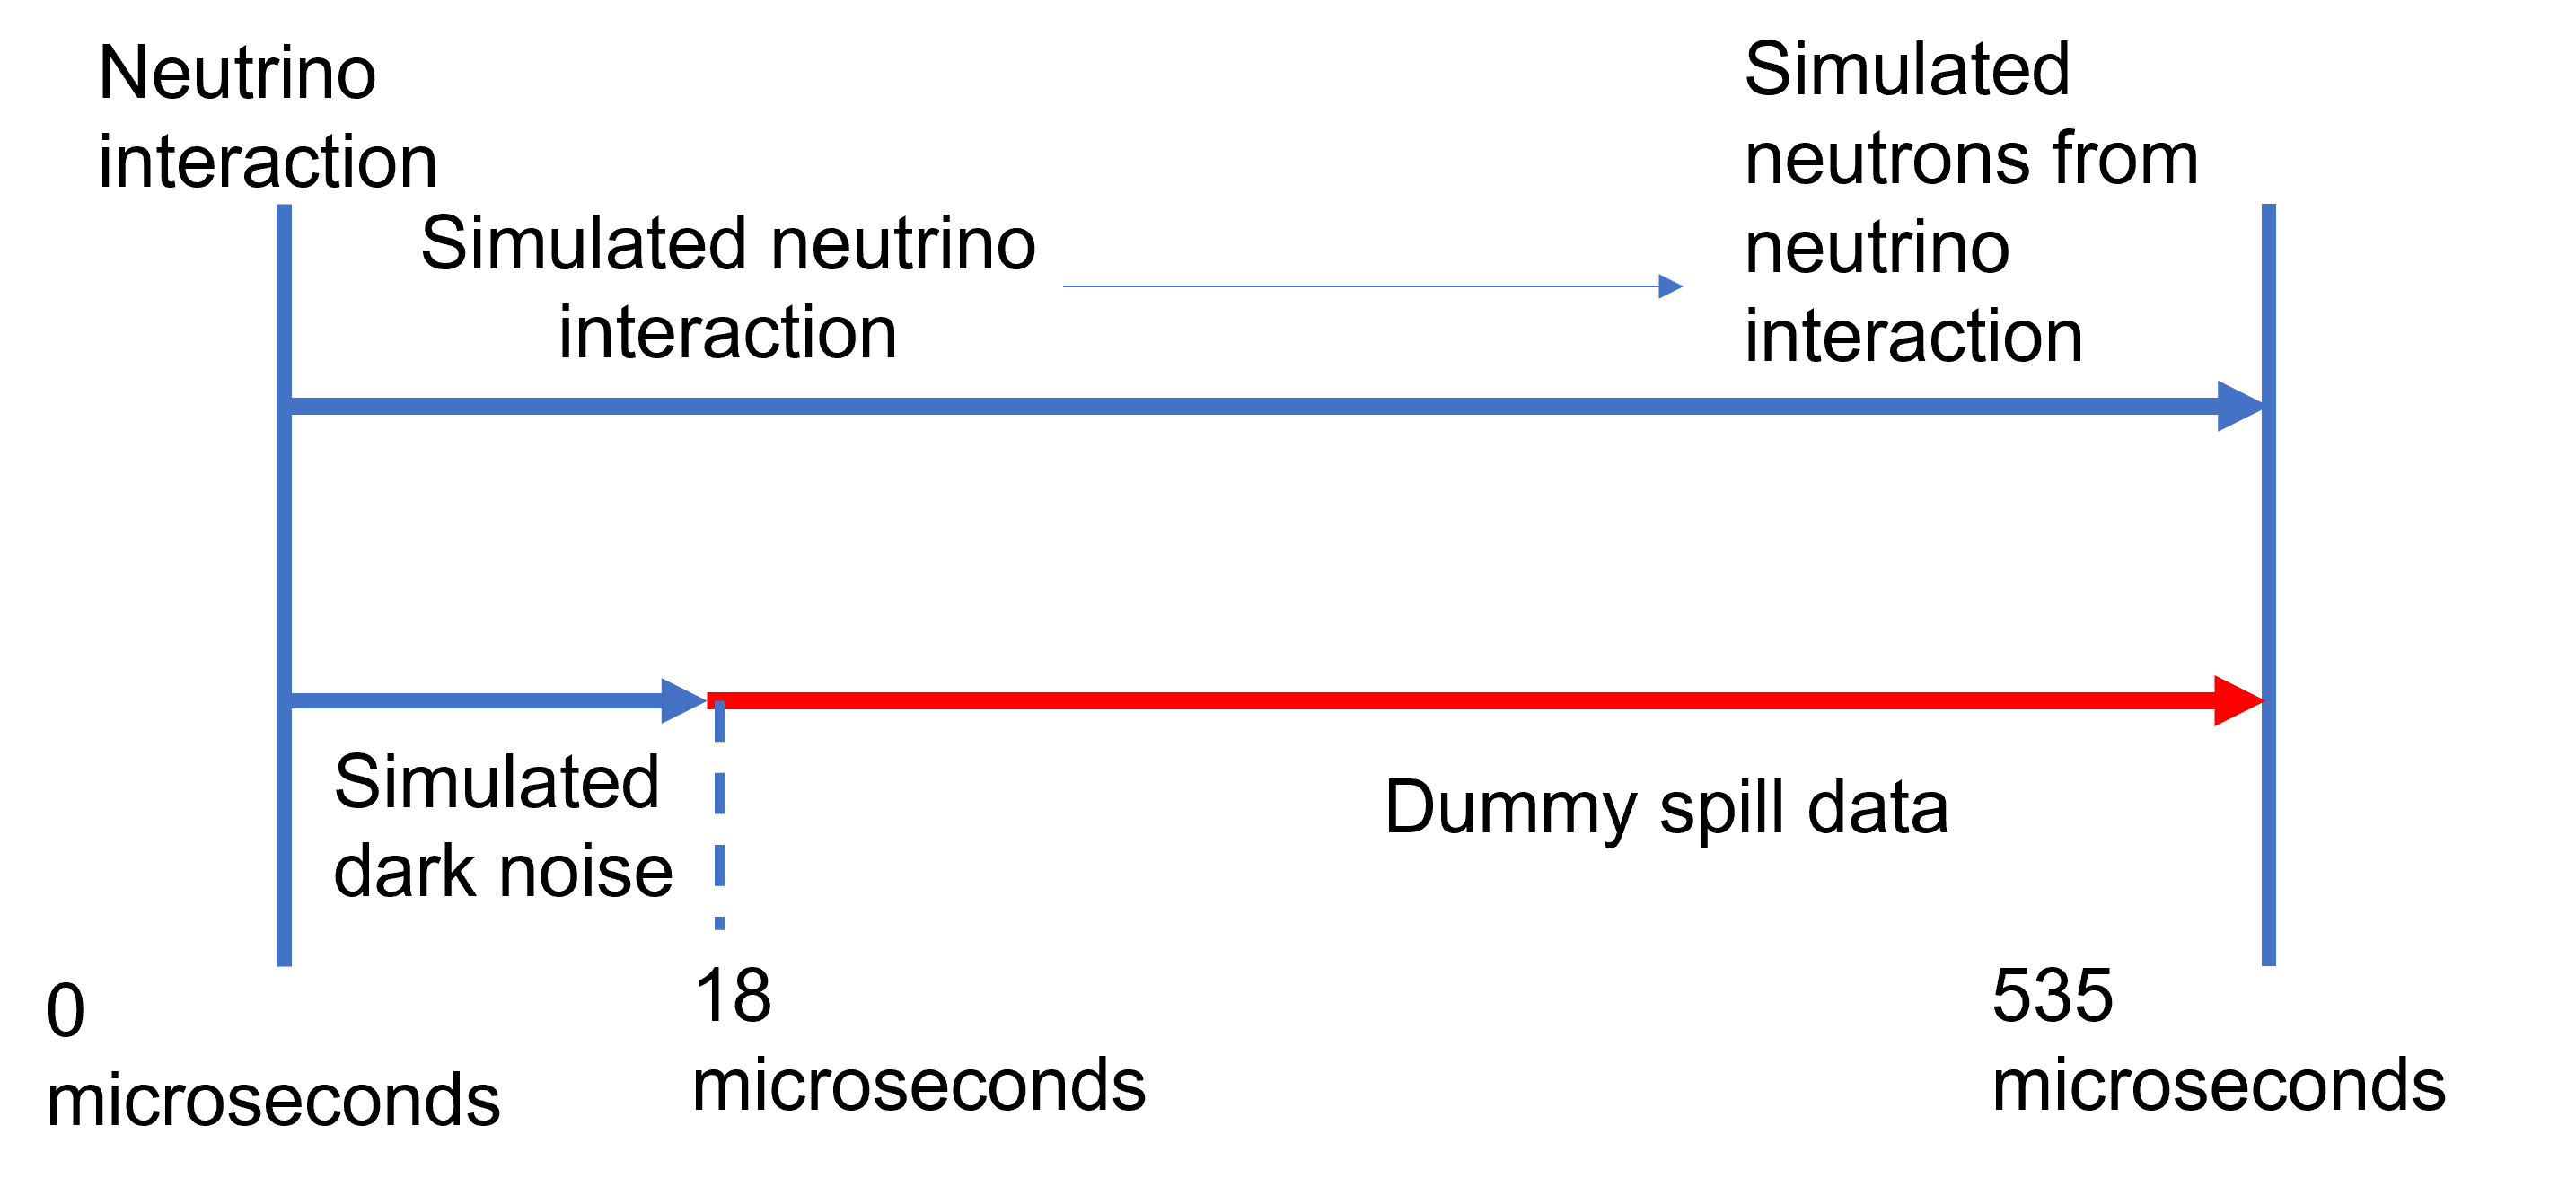
\includegraphics[width=\textwidth]{Figures/dark_rate_schematic.png}
    \caption{Schematic of how dark noise is simulated in this analysis.}
    \label{fig:dark_rate_schematic}

\end{figure}

The reason for the neutron tagging algorithm starting at 18 $\micro$s is in order to take into account the afterpulsing of PMTs, which occurs between 12 $\micro$s and 18 $\micro$s and creates a slight increase in the hit rate, shown in Figure \ref{fig:after_pulsing}, taken from \cite{}. The falling exponential to the left of the after-pulsing peak is caused by decay electrons. 

\begin{figure}

    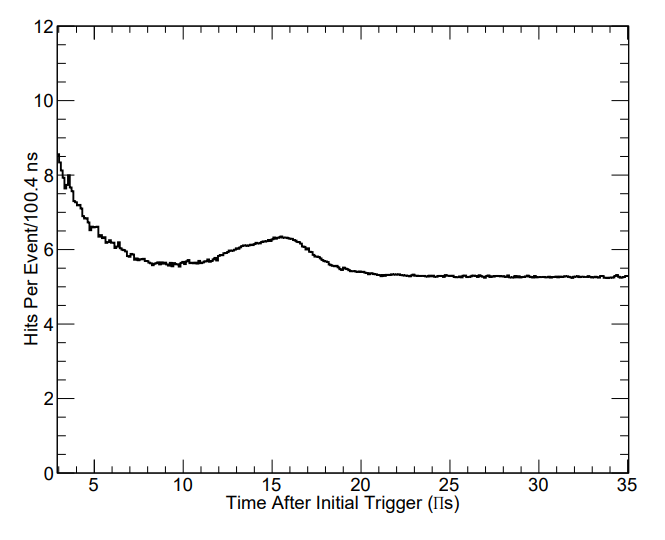
\includegraphics[width=\textwidth]{Figures/after_pulsing.PNG}
    \caption{PMT hit rates per event from the average of events during SK-IV. The after-pulsing peak can clearly be seen in the 12 to 18 $\micro$s region, after which the hit rate is flat for the remainder of the hit window. }
    \label{fig:after_pulsing}

\end{figure}


\section{Secondary selection}

As mentioned previously, two neutron tagging algorithms were used in this analysis, the legacy NTag code, used in previous NCQE analyses and modified to work with a version of SKDETSIM which has Gadolinium included and new NTag code which uses a slightly different neutron tagging algorithm specifically with regards to the primary and secondary selection criteria which will be discussed in later subsections.



\subsection{True neutron tagging information}

Prior to defining the primary and secondary selection criteria for each neutron tagging algorithm, it is important to produce some distributions of basic variables regarding the neutron capture that occur in the simulation, such as neutron capture time, position and number. Figure \ref{fig:NTrueCaptures}, \ref{fig:TrueCaptureTime} show the distribution for the number of neutron captures and the true capture time of the neutrons for both the legacy (green) and new (red) NTag code.  

\begin{figure}
    \centering
     \begin{subfigure}[b]{0.45\linewidth}
      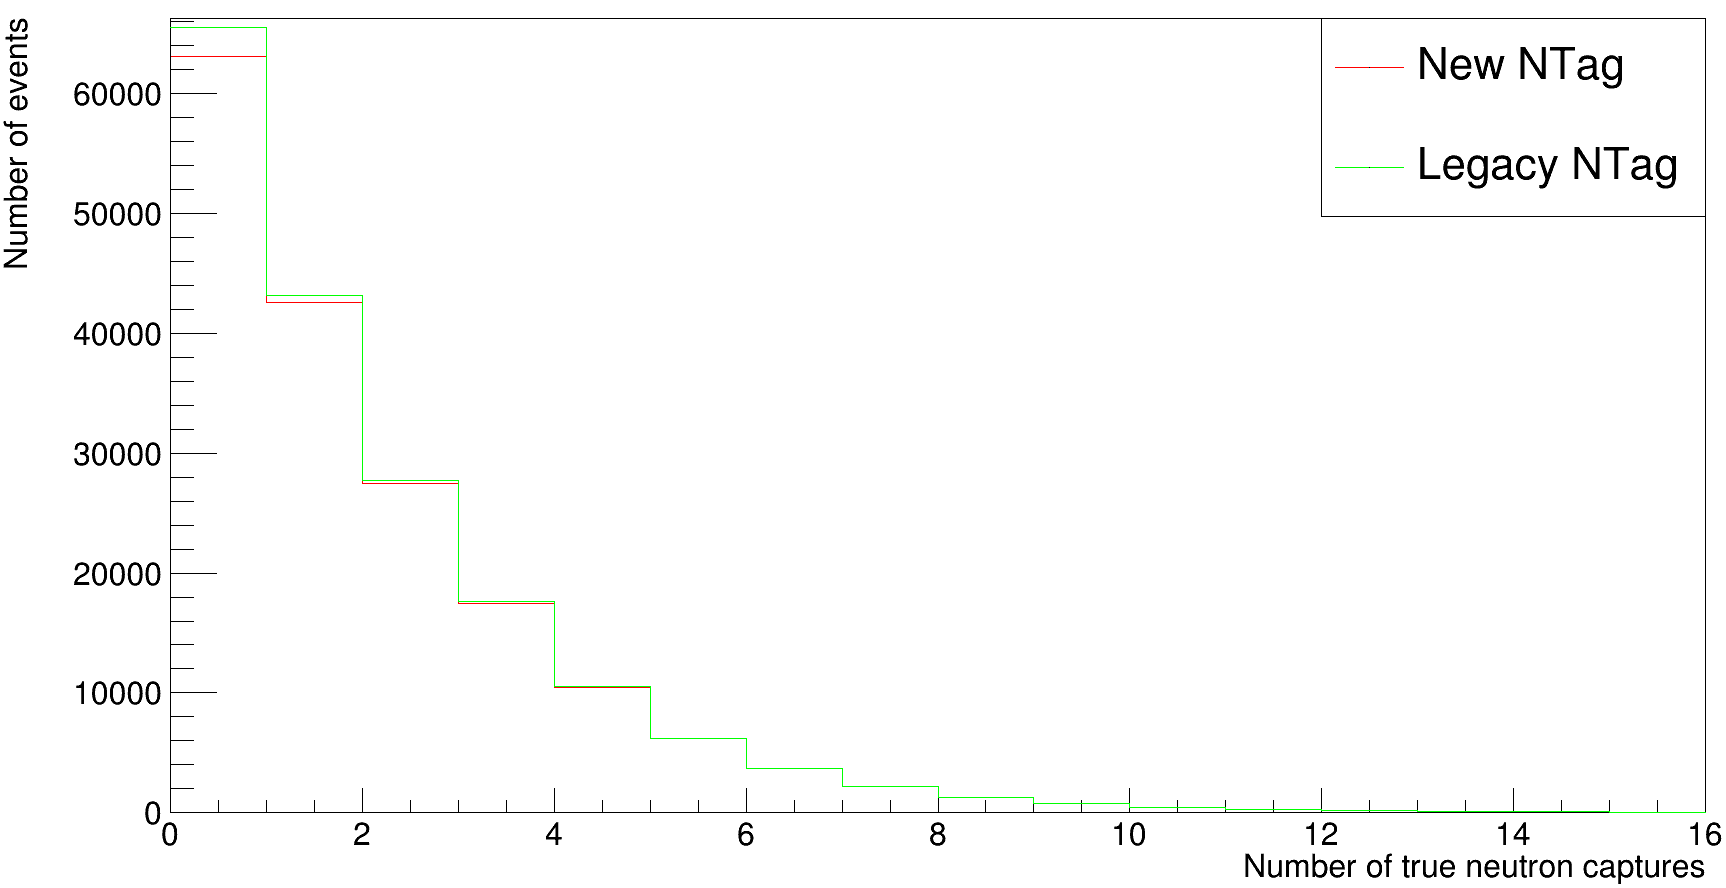
\includegraphics[width=\linewidth]{Figures/NTrueCaptures.PNG}
      \caption{Number of events (y-axis) plotted against number of true neutron captures}
      \label{fig:NTrueCaptures} 
     \end{subfigure}
     \begin{subfigure}[b]{0.45\linewidth}
       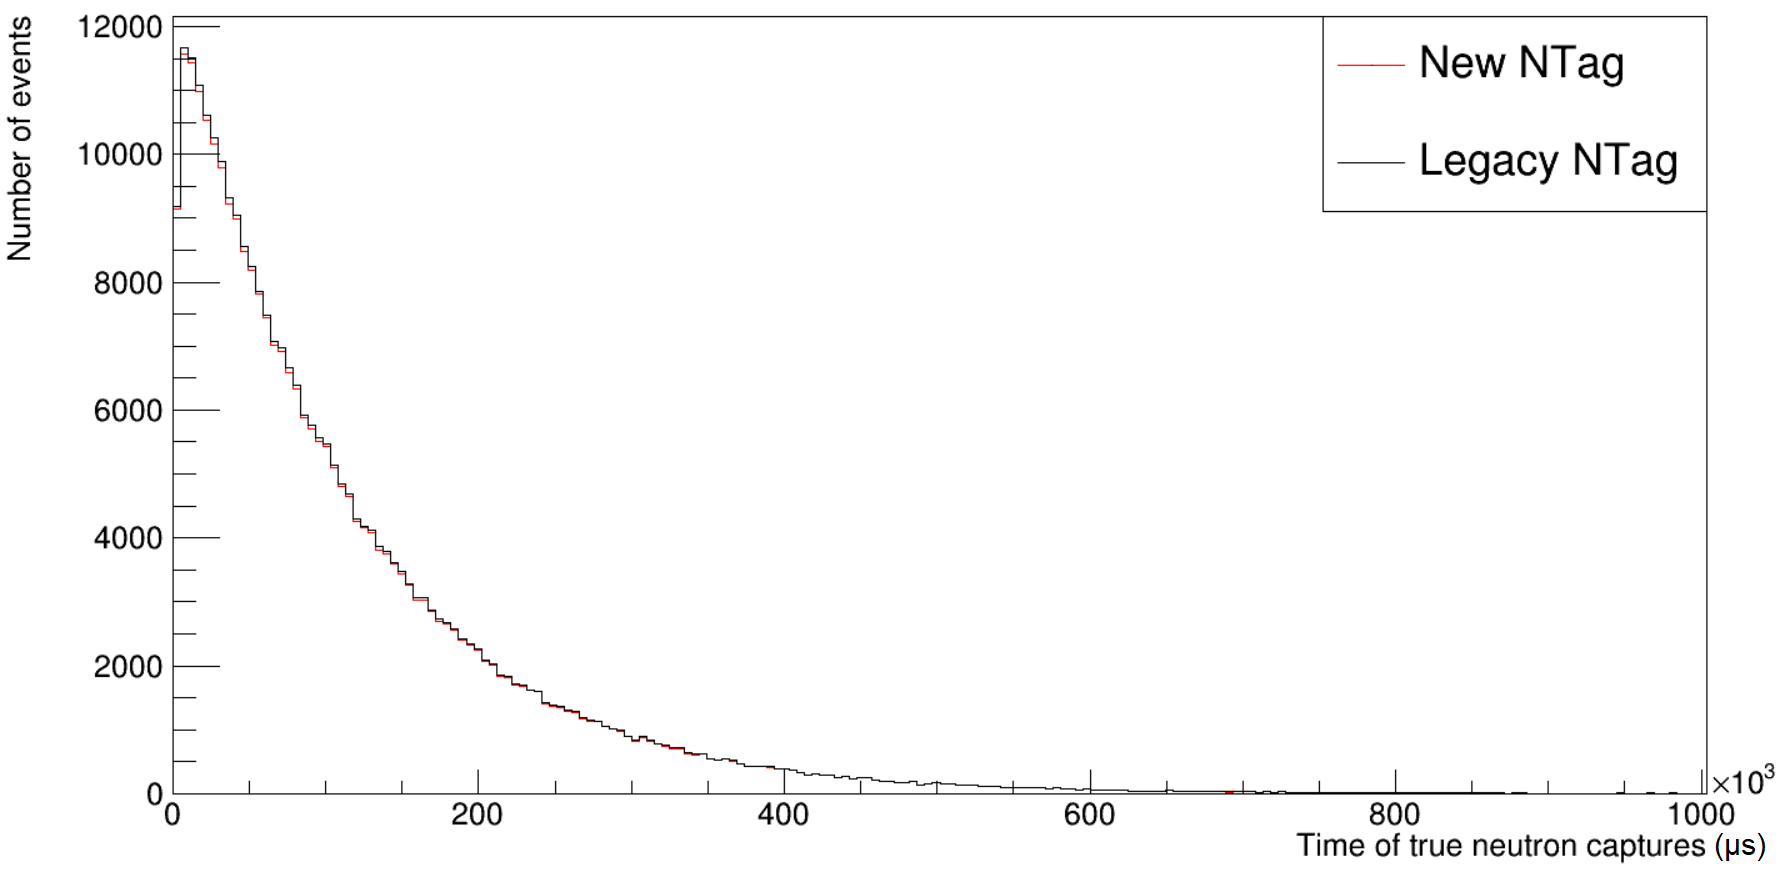
\includegraphics[width=\linewidth]{Figures/TrueCaptureTime.PNG}
        \caption{Number of events (y-axis) plotted against time of all neutron captures in microseconds} 
     \label{fig:TrueCaptureTime}
      \end{subfigure} 
\end{figure}

In order to classify the neutron captures on hydrogen and gadolinium seperately, the energy of the gammas produced from the neutron capture were used, along with the number of gammas produced from the neutron capture. If the energy of the gamma produced is 2.22 MeV and only one gamma ray was produced from the neutron capture, the neutron capture was classified as a capture on Hydrogen. If there are a number of gammas produced in quick succession, the group of gammas is classified as a cascade, and if the energy of the gamma cascade is 8.5 MeV in total it is classified as a neutron capture on  ${ }^{155} \mathrm{Gd}$ and if the energy of the gamma cascade is 7.9 MeV, it is classified as a neutron capture on ${ }^{157} \mathrm{Gd}$. Distributions of the number of gammas produced from neutron capture in the simulation, and also the energy of these gammas were plotted, shown for both the legacy (green) and new (red) NTag code, shown in Figures \ref{fig:NGamma} and \ref{fig:TotGammaE} respectively. 

\begin{figure}
    \centering
     \begin{subfigure}[b]{0.45\linewidth}
      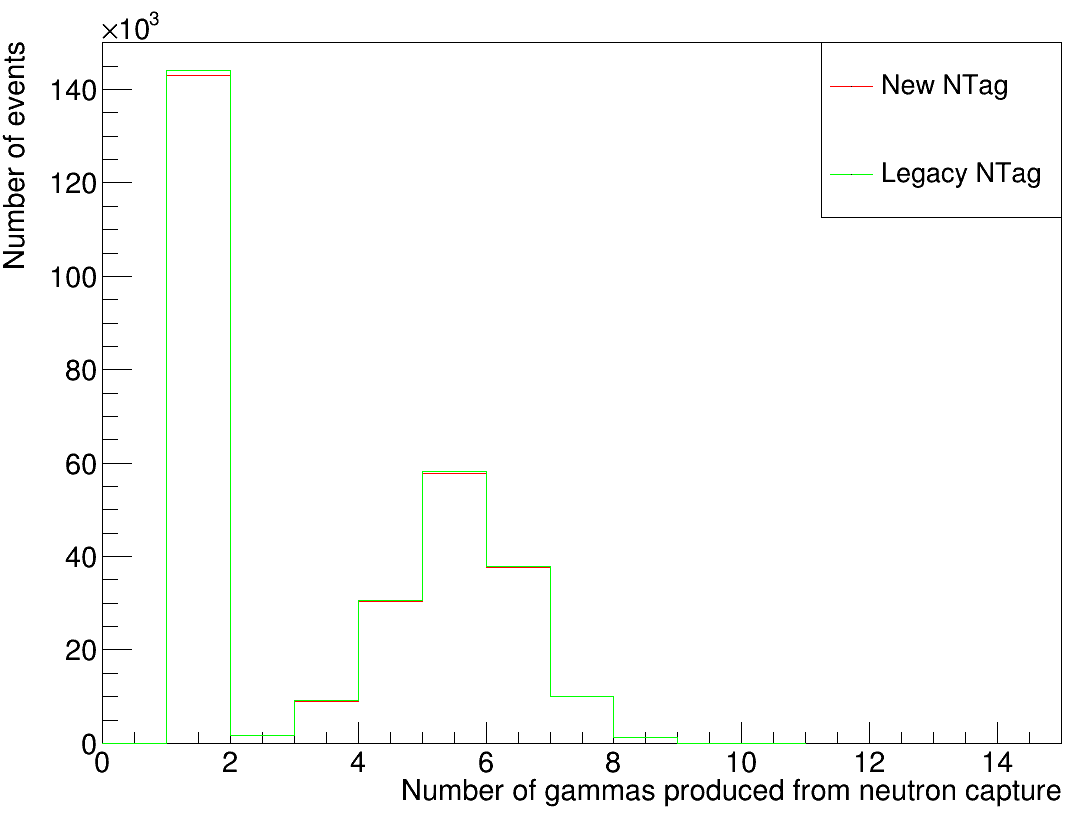
\includegraphics[width=\linewidth]{Figures/NGamma.PNG}
      \caption{Number of events (y-axis) plotted against the number of gammas produced from neutron capture}
      \label{fig:NGamma} 
     \end{subfigure}
     \begin{subfigure}[b]{0.45\linewidth}
       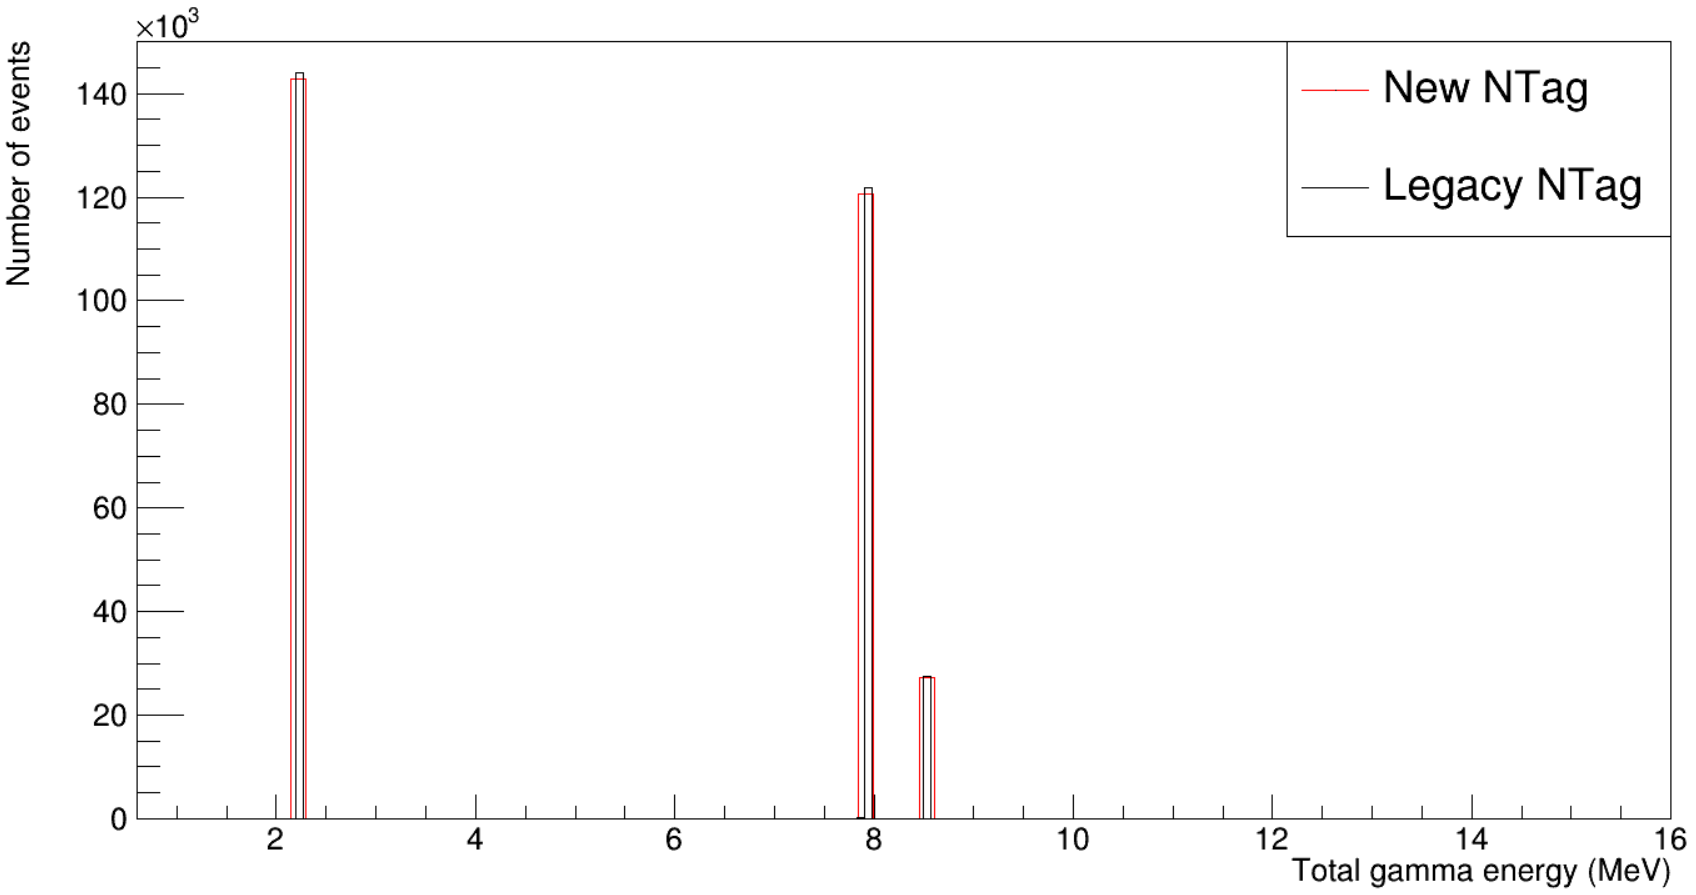
\includegraphics[width=\linewidth]{Figures/TotGammaE.PNG}
        \caption{Number of events (y-axis) plotted against total gamma energy} 
     \label{fig:TotGammaE}
      \end{subfigure} 
\end{figure}

Figure \ref{fig:NGamma} shows that both NTag algorithms have the same number of gammas produced by neutron capture on hydrogen (shown by the peak at 2.22 MeV), and the same number of gammas for the gamma cascade produced by neutron capture on the ${ }^{155} \mathrm{Gd}$ and 
${ }^{157} \mathrm{Gd}$ isotopes of Gadolinium, where the modal number of gammas in the cascade for both NTag code is five. In addition to checking the number and energy of the gammas, and the number and time of true neutron captures, the neutron capture positions for the x,y and z directions were also plotted for Figures \ref{fig:TrueNCapXPos}, \ref{fig:TrueNCapYPos} and \ref{fig:TrueNCapZPos}.


\begin{figure*}
    \centering
     \begin{subfigure}[b]{0.33\linewidth}
      \includegraphics[width=\linewidth]{Figures/TrueNCapXPos.PNG}
      \caption{True neutron capture x-position (cm)}
      \label{fig:TrueNCapXPos} 
     \end{subfigure}%
     \hfill
     \begin{subfigure}[b]{0.33\linewidth}
       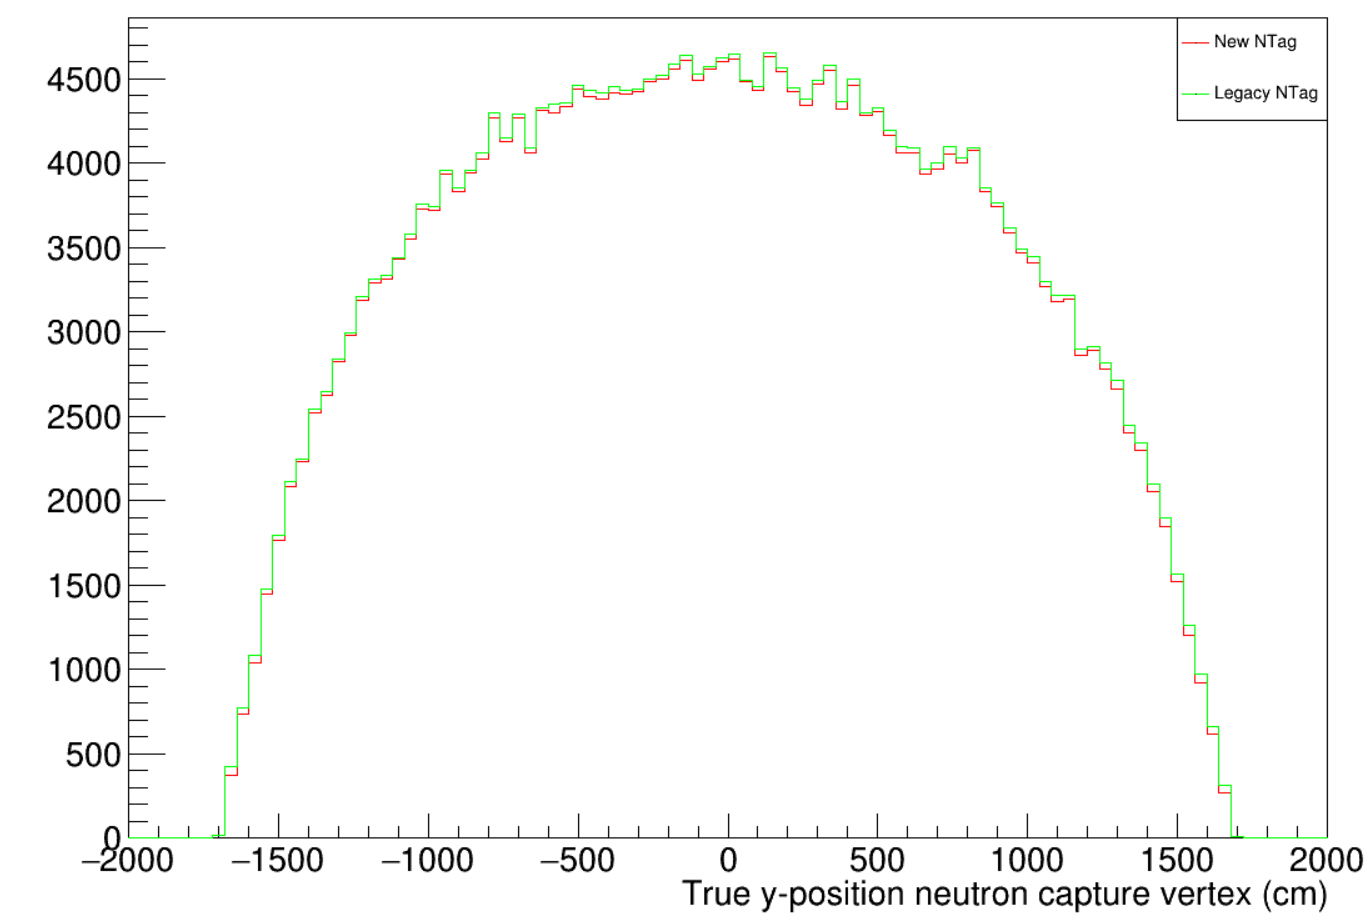
\includegraphics[width=\linewidth]{Figures/TrueNCapYpos.PNG}
        \caption{True neutron capture y-position (cm)} 
     \label{fig:TrueNCapYPos}
      \end{subfigure}% 
      \hfill
      \begin{subfigure}[b]{0.33\linewidth}
      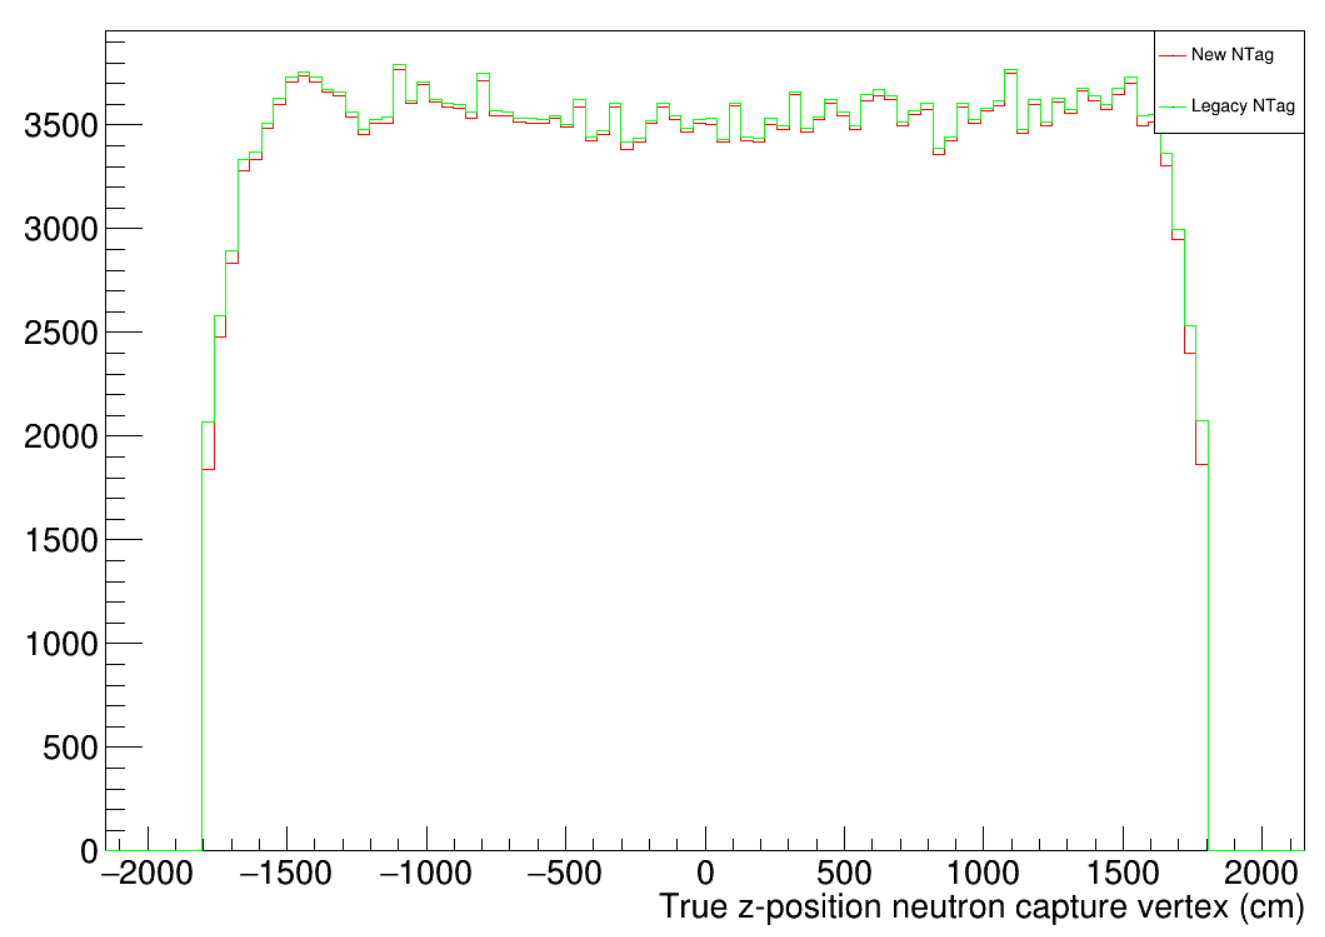
\includegraphics[width=\linewidth]{Figures/TrueNCapZPos.PNG}
      \caption{True neutron capture z-position (cm)}
      \label{fig:TrueNCapZPos}
      \end{subfigure}
\end{figure*}

\subsubsection{Truth information reduction cut plots}

After ensuring that the truth neutron tagging information was the same between the legacy and new NTag versions, the next step was to produce plots with the NCQE reduction cut criteria in order to see the distribution of neutrons for certain variables which satisfy the NCQE criteria. By rewriting aspects of the new NTag code to incorporate the BONSAI variables needed for the NCQE selection, the same reduction cut criteria could be applied to the new NTag code as it was to the new NTag code. Figures \ref{fig:TruCapTimeReductionLegacy} and \ref{fig:TruCapTimeReductionNew} show the number of true neutrons plotted against true neutron capture time for the legacy and new NTag respectively, while Figures \ref{fig:TruCapNuNDistanceReductionLegacy} and \ref{fig:TruCapNuNDistanceReductionNew} show the number of true neutrons plotted against the distance between the true neutron and neutrino capture vertices for the legacy and new NTag respectively.

\begin{figure}
    \centering
     \begin{subfigure}[b]{0.45\linewidth}
      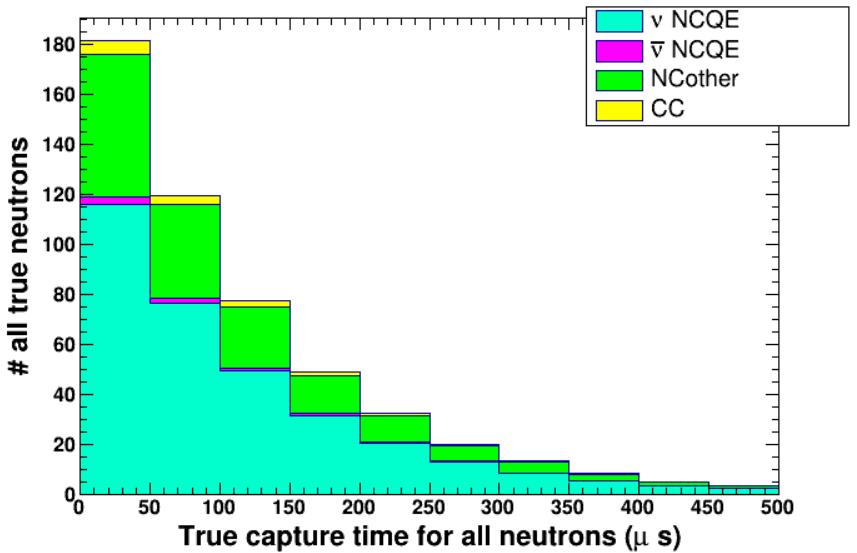
\includegraphics[width=\linewidth]{Figures/TrueCapTimeReductionLegacy.PNG}
      \caption{Number of true neutrons detected plotted against true neutron capture time for the legacy NTag}
      \label{fig:TruCapTimeReductionLegacy} 
     \end{subfigure}
     \begin{subfigure}[b]{0.45\linewidth}
       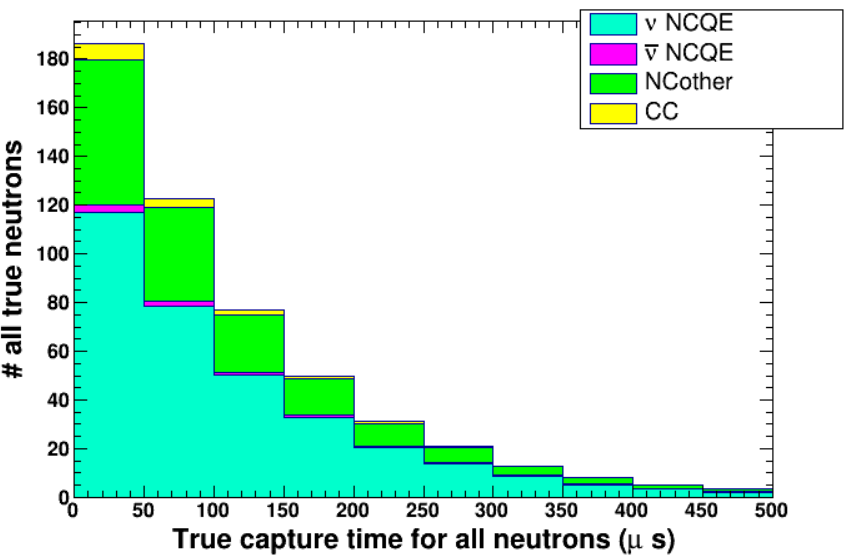
\includegraphics[width=\linewidth]{Figures/TrueCapTimeReductionNew.PNG}
        \caption{Number of true neutrons detected plotted against true neutron capture time for the new NTag } 
     \label{fig:TruCapTimeReductionNew}
      \end{subfigure} 
\end{figure}

\begin{figure}
    \centering
     \begin{subfigure}[b]{0.45\linewidth}
      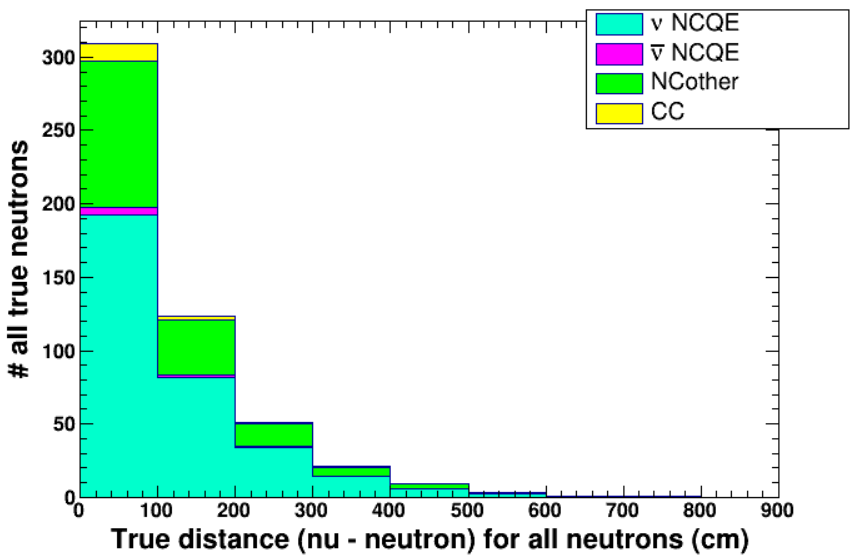
\includegraphics[width=\linewidth]{Figures/TruCapNuNDistanceReductionLegacy.png}
      \caption{Number of true neutrons detected plotted against the distance between the neutrino and neutron capture vertices for the legacy NTag}
      \label{fig:TruCapNuNDistanceReductionLegacy} 
     \end{subfigure}
     \begin{subfigure}[b]{0.45\linewidth}
       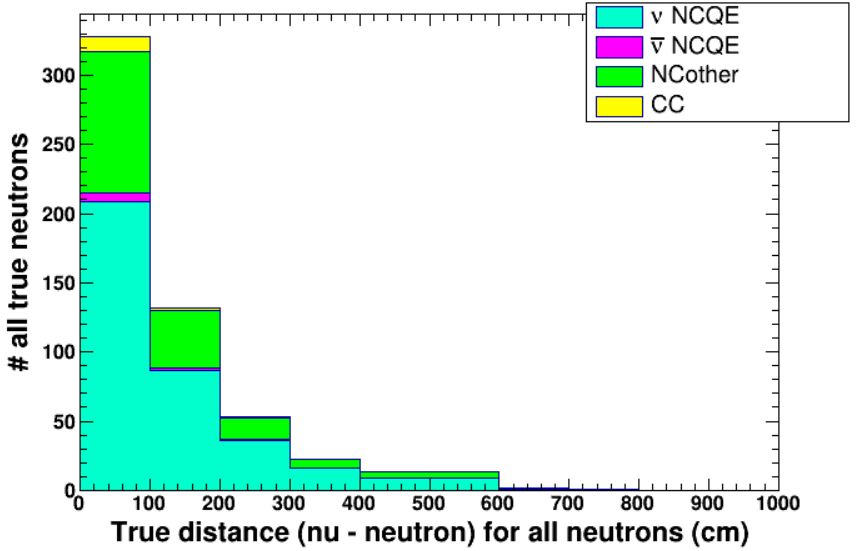
\includegraphics[width=\linewidth]{Figures/TruCapNuNDistanceReductionNew.png}
        \caption{Number of true neutrons detected plotted against the distance between the neutrino and neutron capture vertices for the new NTag } 
     \label{fig:TruCapNuNDistanceReductionNew}
      \end{subfigure} 
\end{figure}

With the level of gadolinium sulphate octahydrate in the simulation, the number of neutron captures on hydrogen and gadolinium should be about half and half. This is confirmed in the plots where the neutron captures in Figures \ref{fig:TruCapNuNDistanceReductionNew} and \ref{fig:TruCapTimeReductionNew} are seperated into captures on hydrogen and gadolinium, shown in Figures \ref{fig:TruCapNuNDistanceReductionNewH}, \ref{fig:TruCapNuNDistanceReductionNewGd}, \ref{fig:TruCapTimeReductionNewH}, \ref{fig:TruCapTimeReductionNewGd}.

\begin{figure}
    \centering
     \begin{subfigure}[b]{0.45\linewidth}
      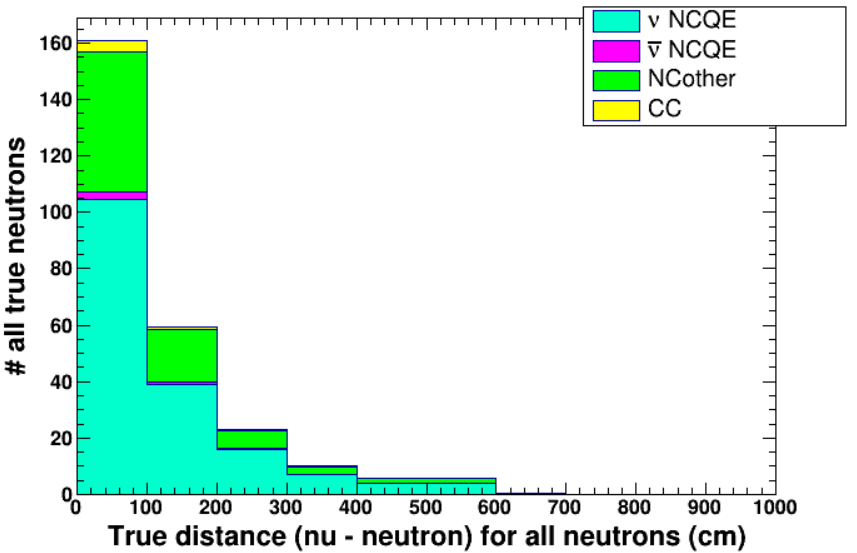
\includegraphics[width=\linewidth]{Figures/TruCapNuNDistanceReductionNewH.PNG}
      \caption{Number of true neutrons detected plotted against the distance between the neutrino and neutron capture vertices for the new NTag, for captures on hydrogen}
      \label{fig:TruCapNuNDistanceReductionNewH} 
     \end{subfigure}
     \begin{subfigure}[b]{0.45\linewidth}
       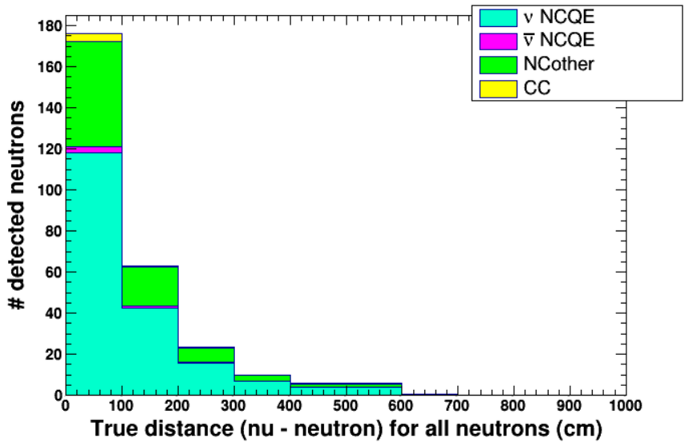
\includegraphics[width=\linewidth]{Figures/TruCapNuNDistanceReductionNewGd.PNG}
        \caption{Number of true neutrons detected plotted against the distance between the neutrino and neutron capture vertices for the new NTag, for captures on gadolinium} 
        \label{fig:TruCapNuNDistanceReductionNewGd}
      \end{subfigure} 
\end{figure}

\begin{figure}
    \centering
     \begin{subfigure}[b]{0.45\linewidth}
      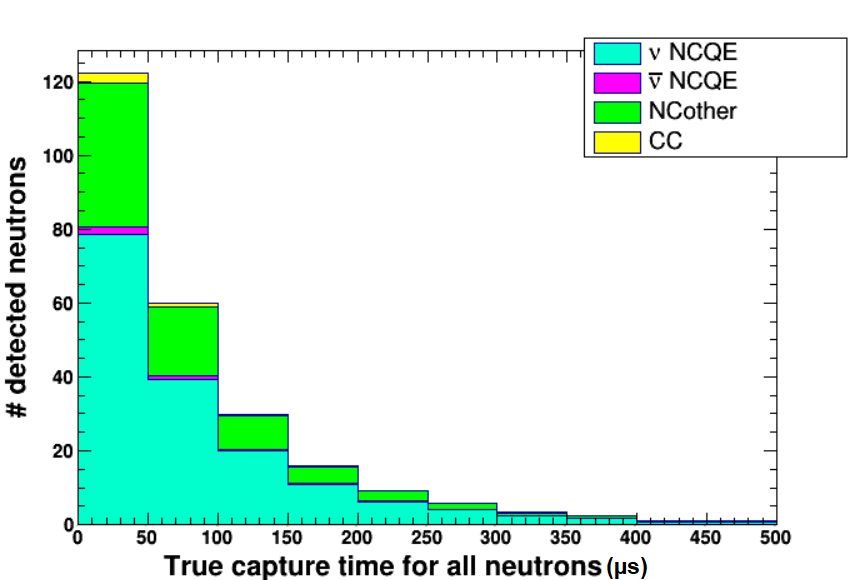
\includegraphics[width=\linewidth]{Figures/TruCapTimeReductionNewH.PNG}
      \caption{Number of true neutrons detected plotted against true neutron capture time for the new NTag, for captures on hydrogen}
      \label{fig:TruCapTimeReductionNewH} 
     \end{subfigure}
     \begin{subfigure}[b]{0.45\linewidth}
       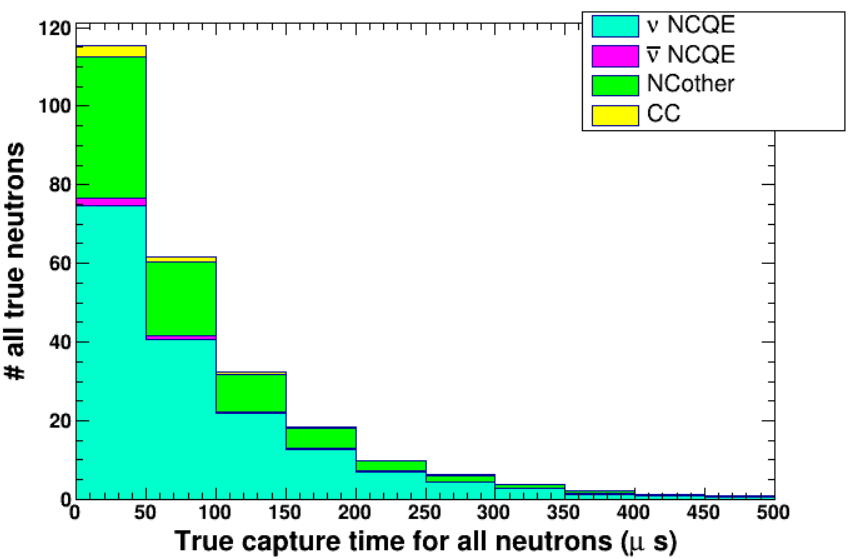
\includegraphics[width=\linewidth]{Figures/TruCapTimeReductionNewGd.PNG}
        \caption{Number of true neutrons detected plotted against true neutron capture time for the new NTag, for captures on gadolinium} 
     \label{fig:TruCapTimeReductionNewGd}
      \end{subfigure} 
\end{figure}


\subsection{Primary selection criteria}

The primary selection criteria are where the differences between the legacy and NTag algorithm come in. What remains constant for both neutron tagging algorithms is firstly, starting the neutron tagging search at 18 $\micro$ s and secondly, the use of calculation of the time of flight corrected PMT hit times as the input into the neutron tagging search window. The reason for calculating the residual time of flight for the gamma hits is because the electrons produced from the Compton scattering of gamma rays produced by the neutron capture on hydrogen and gadolinium appear as a point-like source of Cherenkov radiation. Due to the differing optical path lengths that these photons have, there is a difference in photon hit time. The difference in Cherenkov photon travel length before they hit different PMTs  after the gamma rays from neutron capture Compton scatter off an electron needs to be taken into account via a time-of-flight (TOF) correction. Equation \ref{eq:TOF_correction} gives the equation for the residual hit times $t_{i}^{res}$, where $t_{i}$ is the hit time of the PMTs in the neutron search window and $TOF_{i}$ is given by Equation \ref{eq:TOF_calc}, where $PMT_{i}$ is the position vector of the hit PMT and $VTX_{\nu}$ is the position vector of the reconstructed neutrino vertex and $c_{wt}$ is the speed of light in the medium. The reason $VTX_{\nu}$ is used instead of the Compton scattering vertex is because this vertex is unknown. 

\begin{equation}
    t_i^{\text {res }} \quad=t_i-T O F_i \quad i \in\{\text { Hit PMTs }\}
    \label{eq:TOF_correction}
\end{equation}

\begin{equation}
T O F_i=\frac{\left\|\overrightarrow{P M T_i}-\overrightarrow{V T X_\nu}\right\|}{c_{w t}}
\label{eq:TOF_calc}
\end{equation}

Before the neutron candidate is passed to the secondary selection, other cuts are used to reject candidates which are not neutrons from NCQE interactions. Table \ref{table:legacy_new_selection_criteria} shows the difference between the legacy and new primary selection criteria. The legacy NTag algorithm primary criteria used a 10 nsec sliding window in which hits are searched for a neutron candidate, where the first selection criteria involved making sure the number of hits in the 10 nsec ($N10pvx$) timing window should not exceed 50, and second criteria is that the surrounding window of 200 nsec should not contain more than 100 hits. The third criterion was that in order to avoid double-counting the same 2.2 MeV gamma from neutron capture on hydrogen, each consective neutron candidate must be more than 20 nanoseconds apart. 


\begin{table}
    $$
    \begin{array}{ccc}
    \hline \text{Criterion} & \text{Legacy} & \text{New} \\
    \hline \text { First } & 7 \leq N 10 p v x \leq 50 & 7 \leq NH i t s \leq 400 \\
    \text { Second } & N 200 p v x \leq 100 & N 200 p v x \leq 1000 \\
    \text { Third } & \Delta t_0 \geq 20 \mathrm{nsec} & \Delta t_0 \geq 200 \mathrm{nsec}\\
    \hline
    \end{array}
    $$
    \caption{NTag selection crteria for legacy and new NTag}
    \label{table:legacy_new_selection_criteria}
    \end{table}

The primary selection criteria used with the new NTag are different to accomodate for the fact that a gamma cascade from neutron capture on gadolinium leads to a higher number of hits in the detector. These include increasing the maximum number of hits in the sliding window to 400, and increasing the width of the sliding window from 10 nsec (used with the legacy code) to 14 nsec.  




\subsection{Secondary selection criteria}
Due to the contamination of background events still present amongst the true neutron events after primary selection, a boosted decision tree (BDT) or a neural network (NN) is used to efficiently remove these background events, while trying to maximise the number of true neutron events. The output of the BDT or the NN is used to indicate how likely a variable is to be signal/background candidate. Each of the candidates selected during the primary selection process has an associated reconstructed neutron capture vertex calculated for it. In order to produce residual hit times that are less spread out than TOF-corrected hits towards the neutrino vertex, the TOF-corrected hits towards the Compton scattering vertex are used instead. The aim of searching for the neutron capture vertex is to use a method by which the standard deviation of the residual times of the hits is minimised. Therefore the neutron capture vertex $n_{VTX}$ is for the legacy neutron tagging code is defined as in Equation \ref{eq:ncap_vtx}.

\begin{equation}
    n_{VTX}=\underset{r}{\operatorname{argmin}}\sqrt{\frac{1}{N 10_{p v x}} \sum_{i=1}^{N 10_{p v x}}\left(\tau_i(\boldsymbol{r})-\bar{\tau}(\boldsymbol{r})\right)^2}
\label{eq:ncap_vtx}
\end{equation}

Where $r$ is a trial vertex, the hit time of the $i$-th hit is $t_{i}$, $TOF_{i}(\boldsymbol(r))$, the time-of-flight of the i-th computed hit from the trial vertex, and $\bar{tau}(r)$ is the mean value of the residual time. 

By considering a set of trial vertices on a cubic grid and calculating the standard deviatiation of the residual hit times the minimisation process is performed. After this minimization cycle, a new cycle is performed on a finer and smaller grid and carries on until a certain level of precision is reached. 

When the neutron vertex is found by this method, 14 variables which describe different aspects of the neutron candidate are calculated, using the legacy NTag. For each of the neutron candidates the vector of these variables are computed and fed into the neural network and this produces an output value which is between 0 and 1. These variables relate to different features regarding categorising hits from neutron capture on Gd or H, including the number of the hits from neutron capture, the isotropy of these hits, the Cherenkov angles of these hits and the position of the neutron vertex in the detector when capture occurs. A description of these variables are given as follows for the legacy NTag, and a further 12 variables used in the new NTag code are descibed below.

\underline{Legacy NTag variables}

\underline{N10nvx}
\newline
This is the number of hits in the 10ns sliding window of the neutron candidate.
\newline


\underline{N300S}
\newline
Excluding the number of hits in the 10ns sliding window (N10nvx), this is the number of hits in the extended window of 300ns.
\newline


\underline{NcS}
\newline
This variable is defined as:
\begin{equation}
\label{ncs}
    NcS = N10nvx - Nclushit
\end{equation}

    Where $Nclushit$ is the number of clusterised hits: if hit \textit{i} and \textit{j} are hits on PMTs, then for hit \textit{i} and hit \textit{j} the hit vector $\hat{r}_i$ can be written as:

\begin{equation}
\label{hit}
    \hat{r}_{i}=\frac{\overrightarrow{P M T_{i}}-\overrightarrow{V T X_{n}}}{\left\|\overrightarrow{P M T_{i}}-\overrightarrow{V T X_{n}}\right\|}
\end{equation}

where the angle at the point of the neutron capture vertex between $\hat{r}_{i}$ and $\hat{r}_{j}$ of the PMT hits is defined as:

\begin{equation}
\theta_{i j}=\arccos \left(\hat{p}_{i} \cdot \hat{p}_{j}\right)
\end{equation}

where the hits are defined as clustered if $\theta_{ij}$ is less than 14$\degree$.


\underline{llrca}
\newline
This variable is the log likelihood ratio calculated using triplets of hits from N10nvx that make up a rudimentary Cherenkov cone, from which the opening angle $\theta$ is calculated. Two PDFs ($\theta_{Ci}$) and ($\theta_{Ci}$) are calculated from each $\theta_{Ci}$ where p\_s and p\_b are the probability density functions of $\theta_{C}$ depending on whether the hits come from a true neutron capture on Gd or H or a false neutron capture which makes up the background. The log likelihood ratio variable is computed using Equation {\ref{llrca}}.

\begin{equation}
\label{llrca}
\newline
  llrca =\sum_{i \in\{ { triplets }\}} \log \left(\frac{f_{B}\left(\theta_{C i}\right)}{f_{S}\left(\theta_{C i}\right)}\right)
\end{equation}


\underline{beta-n}
\newline
These variables (where n = 1,2,3,4,5) are defined using Legendre polynomials, shown in Equation \ref{beta}, which gives the isotropy of the Cherenkov hits.

\begin{equation}
\label{beta}
 beta- n=\frac{2}{N 10 {nvx}(N 10 {nvx}-1)} \sum_{i \neq j}  { Legendre }_{n}\left(\cos \theta_{i j}\right)
\end{equation}

where $Legendre_n$ gives the Legendre polynomial of order $n$ and $theta_{ij}$ is the angle between hit PMTs relative to the neutron capture vertex.



\underline{ndwall}
\newline
This parameter, similar to dwall, gives the shortest distance of the neutron capture vertex from the wall of the Super-Kamiokande tank.
\newline



\underline{ntowall}
\newline
This variable (similar to effwall), gives the distance of the neutron capture vertex from the wall, however, unlike ndwall it gives the direction of the neutron capture specifically along the direction of the centre of the hits. The direction ($\overrightarrow{R}$) is given by:

\begin{equation}
\overrightarrow{\operatorname{dir}}=\sum_{i=1}^{N 10 n v x} \hat{p}_{i}
\end{equation}

\underline{accepave}

This is a variable that relates to the acceptance of the inner detector PMTs. For every ID PMT the geometric acceptance angle is defined as: 

\begin{equation}
    \cos \theta=\hat{n} \cdot\left(\overrightarrow{V T X_n}-\overrightarrow{P M T}\right) 
\end{equation}

where $\cos \theta=\hat{n} \cdot\left(\overrightarrow{V T X_n}-\overrightarrow{P M T}\right)$ is the vector between the neutron capture vertex to the hit PMT, and $hat{n}$ is a unit vector orthogonal to the PMT cover. Using the cosine of these acceptance values, weights are computed using 


\begin{equation}
    w^*=(\cos \theta)_{e f f} \times \frac{e^{-d / \lambda}}{d^2}
\end{equation}

where $(\cos \theta)_{e f f}$ is $\cos \theta$ corrected for imperfections resulting from PMT geometry and light being reflected and absorbed by the acrylic PMT cases, while the multiplicative term consisting of $d = \left(\overrightarrow{V T X_n}-\overrightarrow{P M T}\right)$, and adjust the weight by looking at the attenuation length of the Cherenkov photon in water ($\lambda$). Min-max normalising the $w^{*}$ weights produces the weights $w$ so that the values of $w$ never exceed 1. The formula for the $accepave$ variable is finally given by:

\begin{equation}
    \text { accepave }=-\frac{1}{N 10 n v x} \sum_{i=1}^{N 10 n v x} \log _{10}\left(\frac{w_i}{\sum_{i=1}^{N_{P M T}} w_i}\right)
\end{equation}

\underline{taurms}

This is a variable relating to the timing of the hits, specifically the standard deviation of the time-of-flight corrected hit times of the candidate event ($\sigma_{res}$).

\underline{mintaurms6}

This is another variable related to hit timing, and is the minimum value among the values of $\sigma_{res}$ from all possible subsets of six hits taken from the neutron candidate. 

\underline{New NTag variables}

The following twelve variables are fed into the TMVA neural network model for the secondary selection, some of these are similar to their corresponding legacy NTag variables, while some are new additions. 

\underline{NHits}

Similarly to the legacy NTag variable $N10nvx$ this is defined as the number of hits in a sliding timing window for the neutron candidate, however instead of this being set to a value of 10 nsec, this was increased to 14 nsec in order to accomadate for the increased number of hits from gamma cascades from neutron capture on gadolinium.

\underline{Beta-L}

Again, similarly to the $beta-n$ variable of the legacy NTag, this defines the isotropy of the Cherenkov hits according to:

\begin{equation}
    \beta_l=\frac{2}{N_{H i t s}\left(N_{H i t s}-1\right)} \sum_{i \neq j} P_l\left(\cos \theta_{i j}\right)
\end{equation}

where the legacy NTag variable $N10nvx$ is replaced by $N_{Hits}$, and $P_{l}$ are the Legendre polynomial's of order $l$ and $\theta_{ij}$ is the angle between hit PMTs relative to the neutron capture vertex.

\underline{DWall}

DWall gives the difference from the fitted neutron vertex to the nearest wall in cm.

\underline{DWallMeanDir}

Similarly to the variable ntowall, this gives the distance from the fitted neutron vertex to the wall in the direction of the mean of the PMT hits for the neutron candidate in cm.

\underline{MeanDirAngleMean}

Unlike the legacy NTag, which uses the variables $accepave$ and $llrca$ relating to hits spacing that involve complicated weighting of PMT acceptance angles and log-likelihood ratios of Cherenkov angles, this variable simply takes the mean of angles between the direction of each hit and the mean of the direction of these hits. 

\underline{MeanDirAngleRMS}

This variable is simply the RMS of angles between each hit directon and mean hit direction.

\underline{OpeningAngleMean}

This calculates the mean of all possible opening angles calculated from 3 PMT hits.

\underline{OpeningAngleStdev}

This is the standard deviation of all possible opening angles calculated from 3 PMT hits.

\underline{OpeningAngleSkew}

This is the skewness of all possible opening angles from 3 PMT hits, calculated using

\begin{equation}
    \tilde{\mu}_3=\frac{\sum_i^N\left(X_i-\bar{X}\right)^3}{(N-1) * \sigma^1.5}
\end{equation}

where $X_{i}$ is the hit PMT, $\bar{X}$ is the mean of the 3-hit vector, N is the size of the vector of PMT hits, and $\sigma$ is the standard deviation of the PMT hits.

\underline{TRMS}

Similarly to the legacy NTag variable $taurms$, this calculates the standard deviation of the time-of-flight corrected PMT hit times.

\underline{N1300}

Just like the variable $N300S$ from the legacy NTag, this is a broader range timing window than NHits, this is the number of PMT hits in a 1300 ns timing window, specifically between -520 ns and +780 ns from the fitted time relative to the trigger.       

\underline{N200}

This is the number of hits within -100 ns and +100 ns from the fitted time relative to the trigger.


